\documentclass[12pt,a4paper]{article}
\topmargin -1.6cm
\addtolength{\textheight}{4cm}
\textwidth  15.5cm

\leftmargin      5mm
\rightmargin     5mm
\oddsidemargin   5mm
\evensidemargin  5mm

\usepackage{hyperref}
\usepackage{polski}
\usepackage[utf8]{inputenc}
\usepackage{graphicx}
\usepackage{units}
\usepackage{sty/style}
\usepackage{float}

\projekt{Sterowanie obiektem nieholonomicznym}
\autor{Marcin Bober, 249426}
\przedmiot{Projekt specjalnościowy ARR}
\prowadzacy{Dr inż. Mirela Kaczmarek}

\begin{document}
\pdfpageheight   297mm
\pdfpagewidth    210mm

\StronaTytulowa
\SpisTresci

\pagebreak

\section{Cel ćwiczenia}
  Celem ćwiczenia jest zbadanie i porównanie zachowania obiektu nieholonomicznego sterowanego na dwa sposoby. W sposób czysto kinematyczny oraz kinematyczny i dynamiczny zarazem. W obu przypadkach celem sterowania jest śledzenie trajektorii. Wykorzystany w tym celu zostanie algorytm Samsona dla części kinematycznej oraz algorytm dokładnej linearyzacji dla części dynamicznej.

  % algorytm samsona jest kinematyczny. produjeje profil prędkościowy zależny od zadania. informacja z niego wykorzystywana jest w dynamicznym. 

  % w dynamicznym używamy algorytmu dokładnej linearyzacji

  % k1, k2 kinematyczny, 
  % km = 1-10


  % kinematyczny produjeje profil prędkościowy zależny od zadania, dynamiczny wymusza zbierzność prędkości do prędkości referencyjnej. 


\section{Sterownik kinematyczny}
  W tym doświadczeniu do obiektu został podpięty jedynie sterownik kinematyczny. Wyniki błędów referencyjnych śledzenia trajektorii zostały zaprezentowane na wykresie \ref{fig:1}. Trajektoria po której poruszał się obiekt jest przedstawione na wykresie \ref{fig:2}.

  \begin{figure}[H]
    \centering
    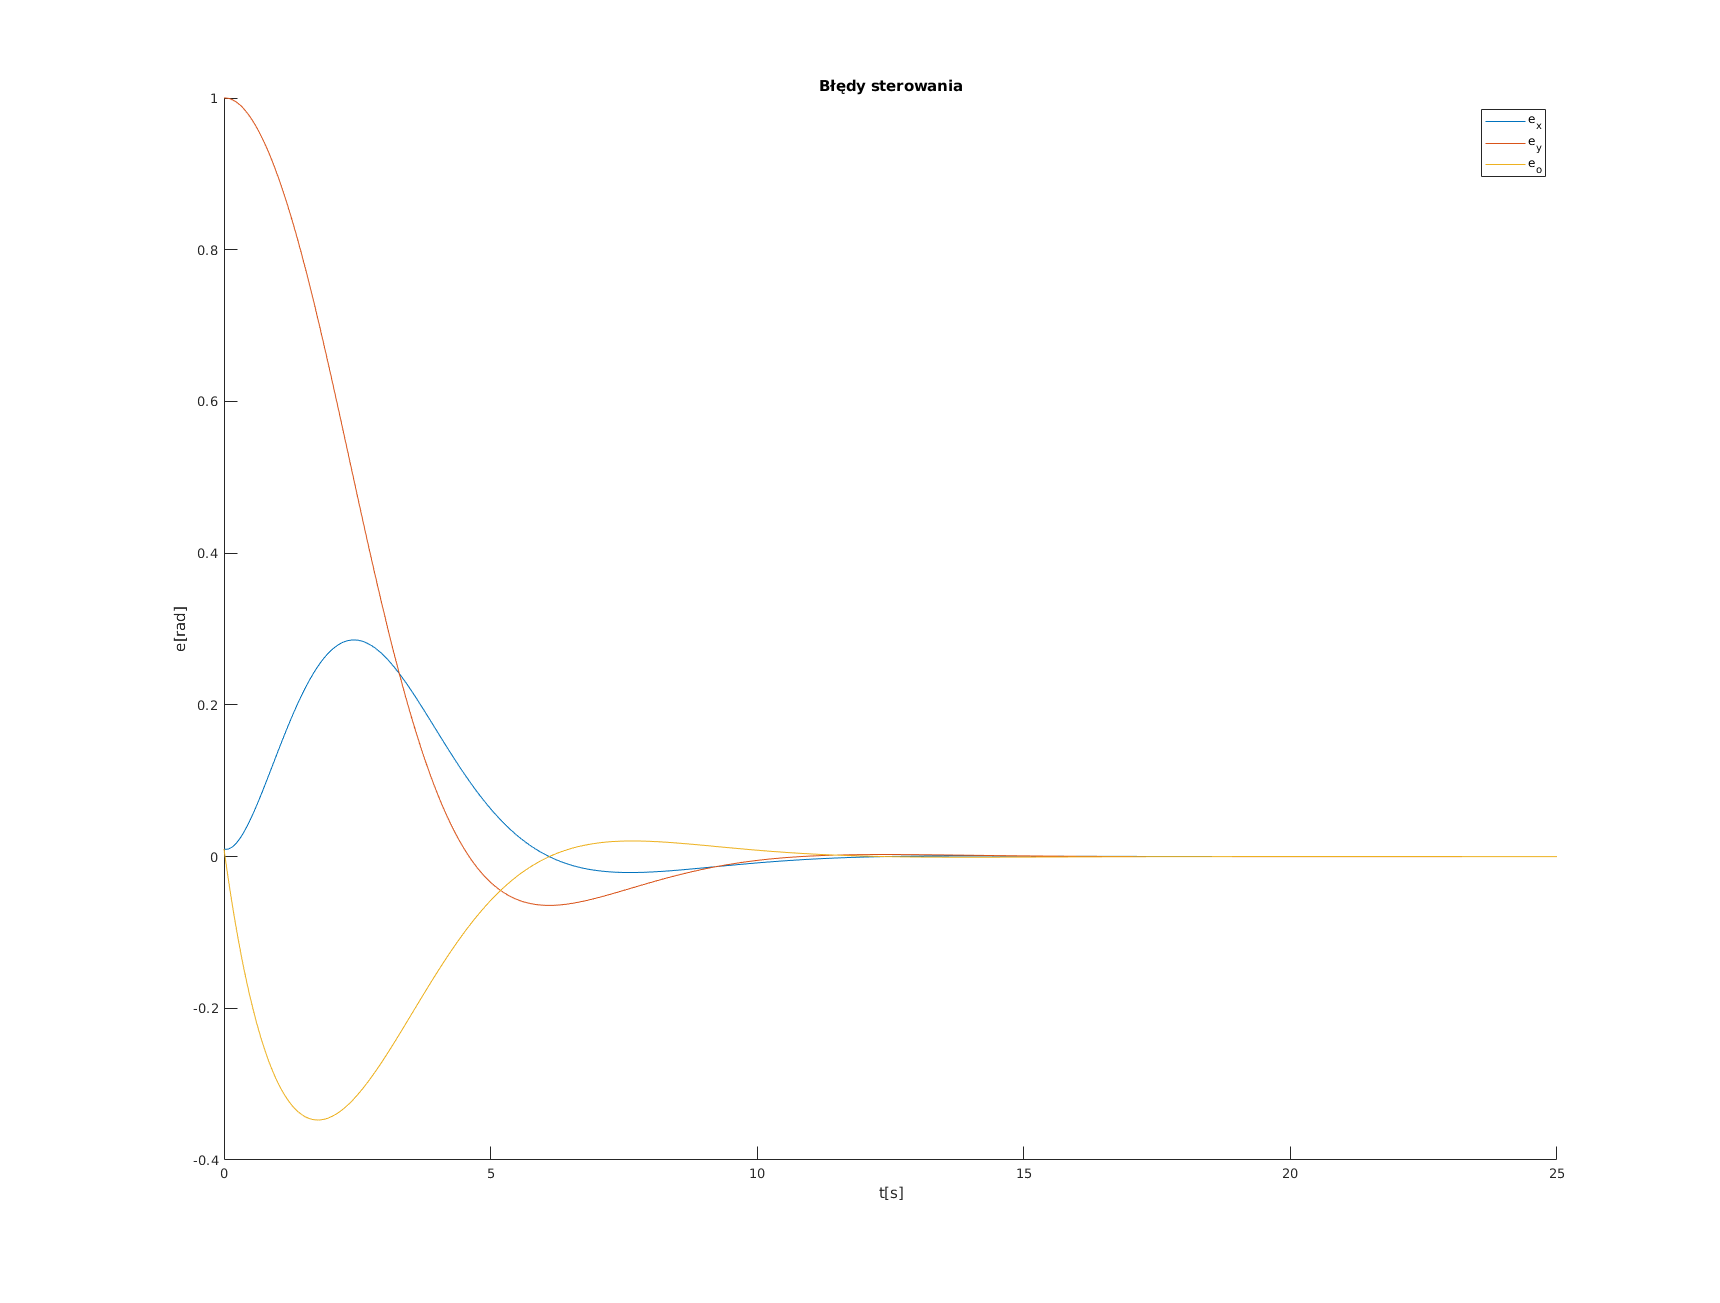
\includegraphics[width=1\textwidth]{figures/kin_bledy.png}
    \caption{Błędy $e_x$, $e_y$, $e_\theta$}
    \label{fig:1}
  \end{figure}

  \begin{figure}[H]
    \centering
    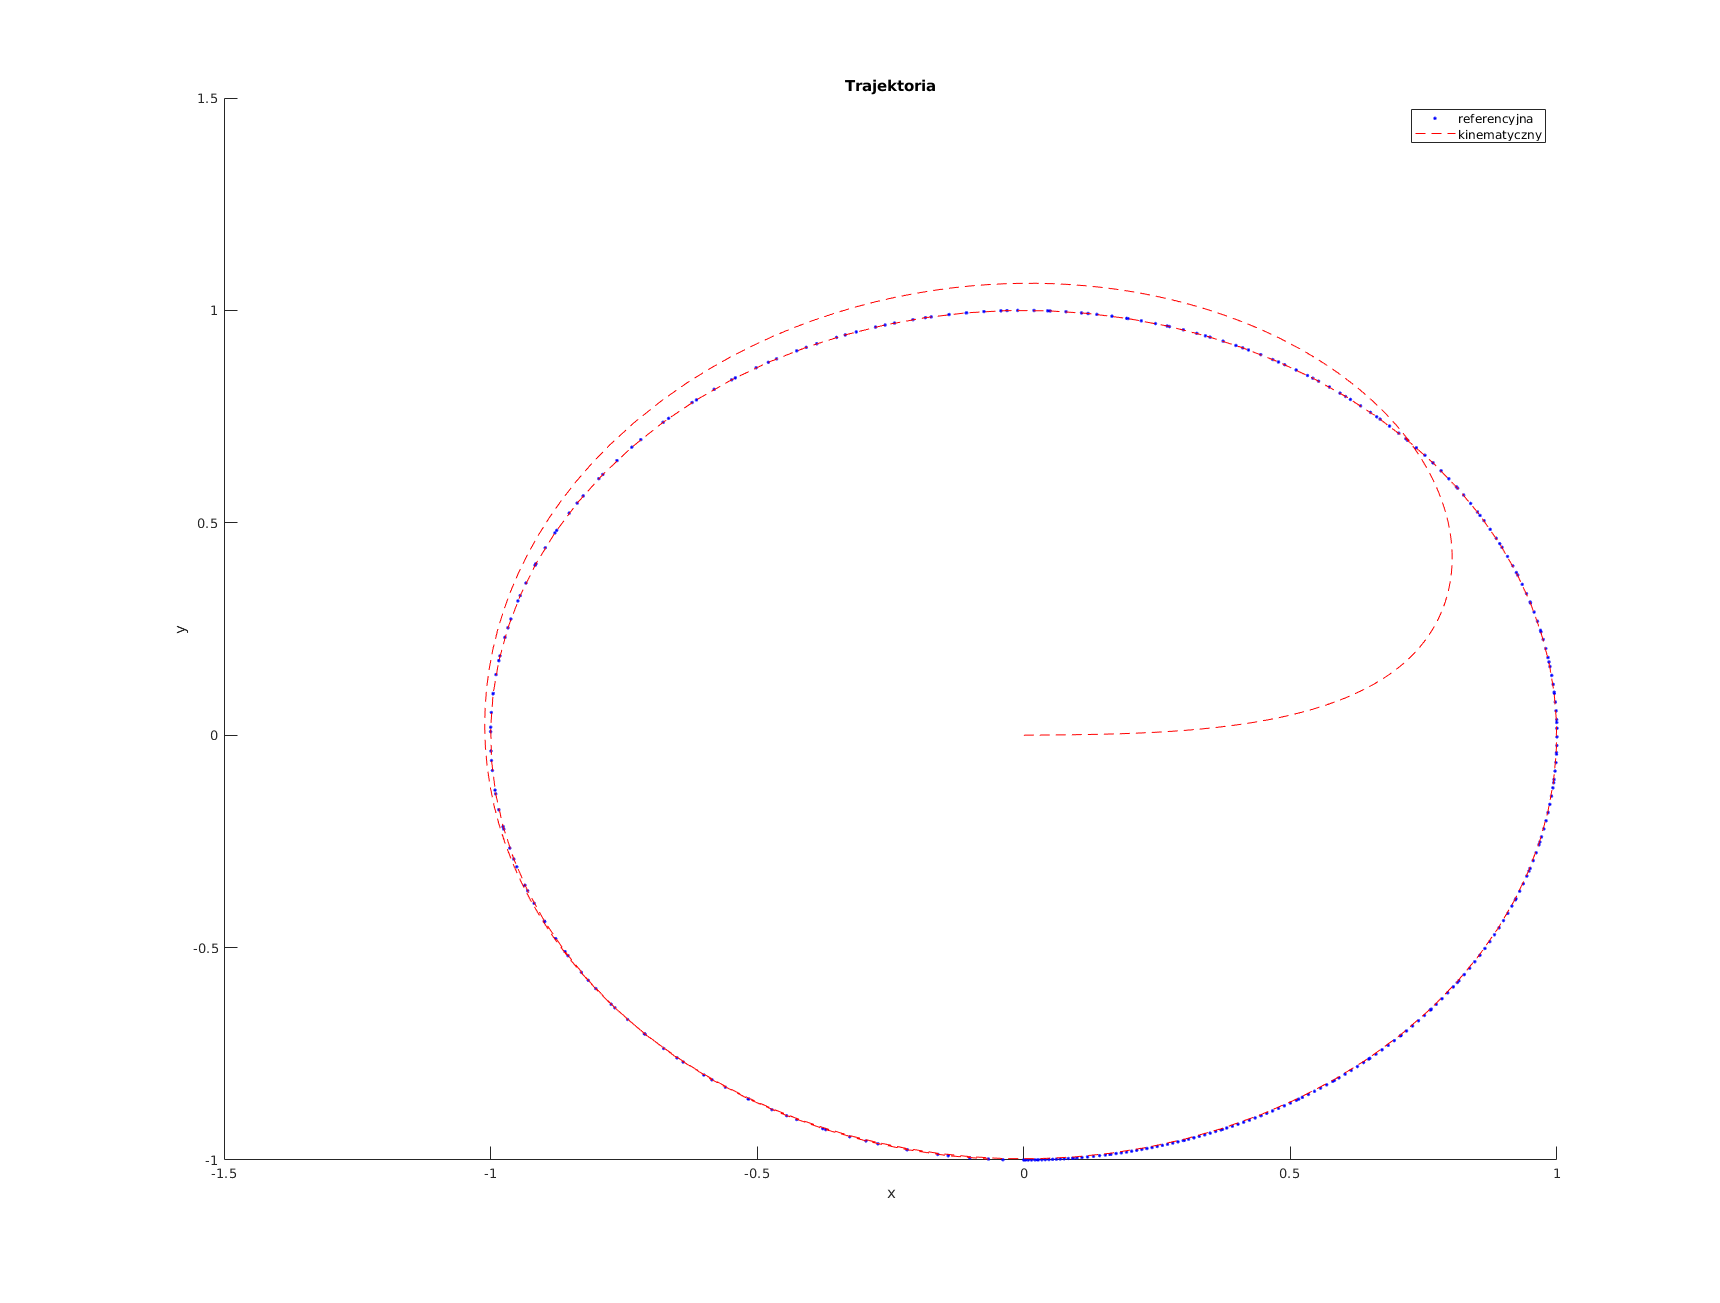
\includegraphics[width=1\textwidth]{figures/kin_trajektoria.png}
    \caption{Trajektoria}
    \label{fig:2}
  \end{figure}


\section{Sterownik kinematyczny i dynamiczny}

  \subsection{Błędy śledzenia trajektorii}
    Eksperyment ten zakłada wykorzystanie dwóch sterowników kinematycznego i dynamicznego jednocześnie. Profil prędkościowy produkowany przez sterownik kinematyczny jest wykorzystywany przez sterownik dynamiczny, którego zadaniem jest minimalizacja błędów śledzenia trajektorii.

    \begin{figure}[H]
      \centering
      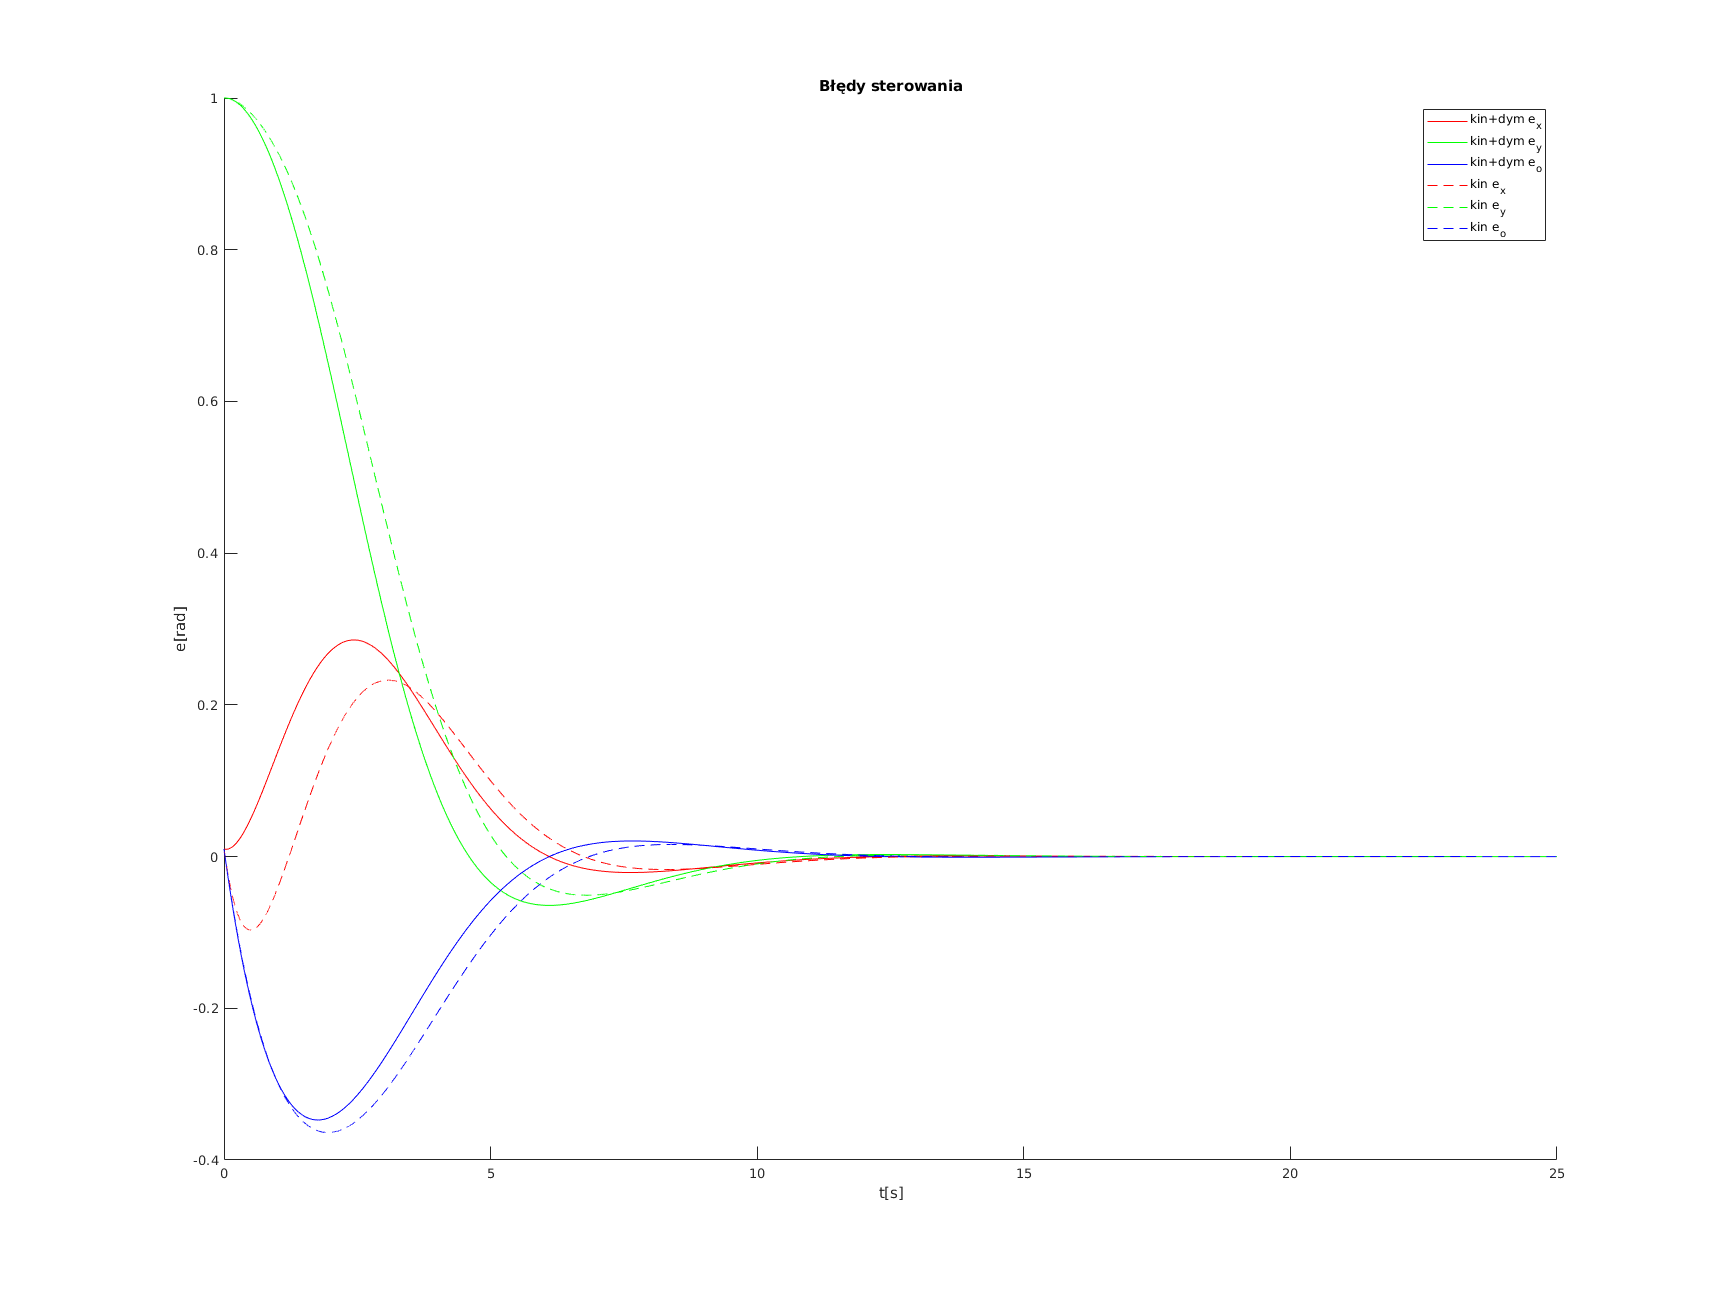
\includegraphics[width=1\textwidth]{figures/dyn_bledy.png}
      \caption{Błędy $e_x$, $e_y$, $e_\theta$}
      \label{fig:3}
    \end{figure}

    Na wykresie \ref{fig:3} można zaobserwować odnotowane błędy śledzenia trajektorii. Liniami ciągłymi oznaczone są błędy dotyczące sterownika kinematycznego, natomiast liniami przerywanymi rysowane są wykresy dotyczące połączenia oby sterowników. Można zaobserwować że połączenie obu sterowników daje wymiernie lepsze efekty. Połączenie sterowników pozwala szybciej i intensywniej reagować na pojawiający się błąd. 

    \begin{figure}[H]
      \centering
      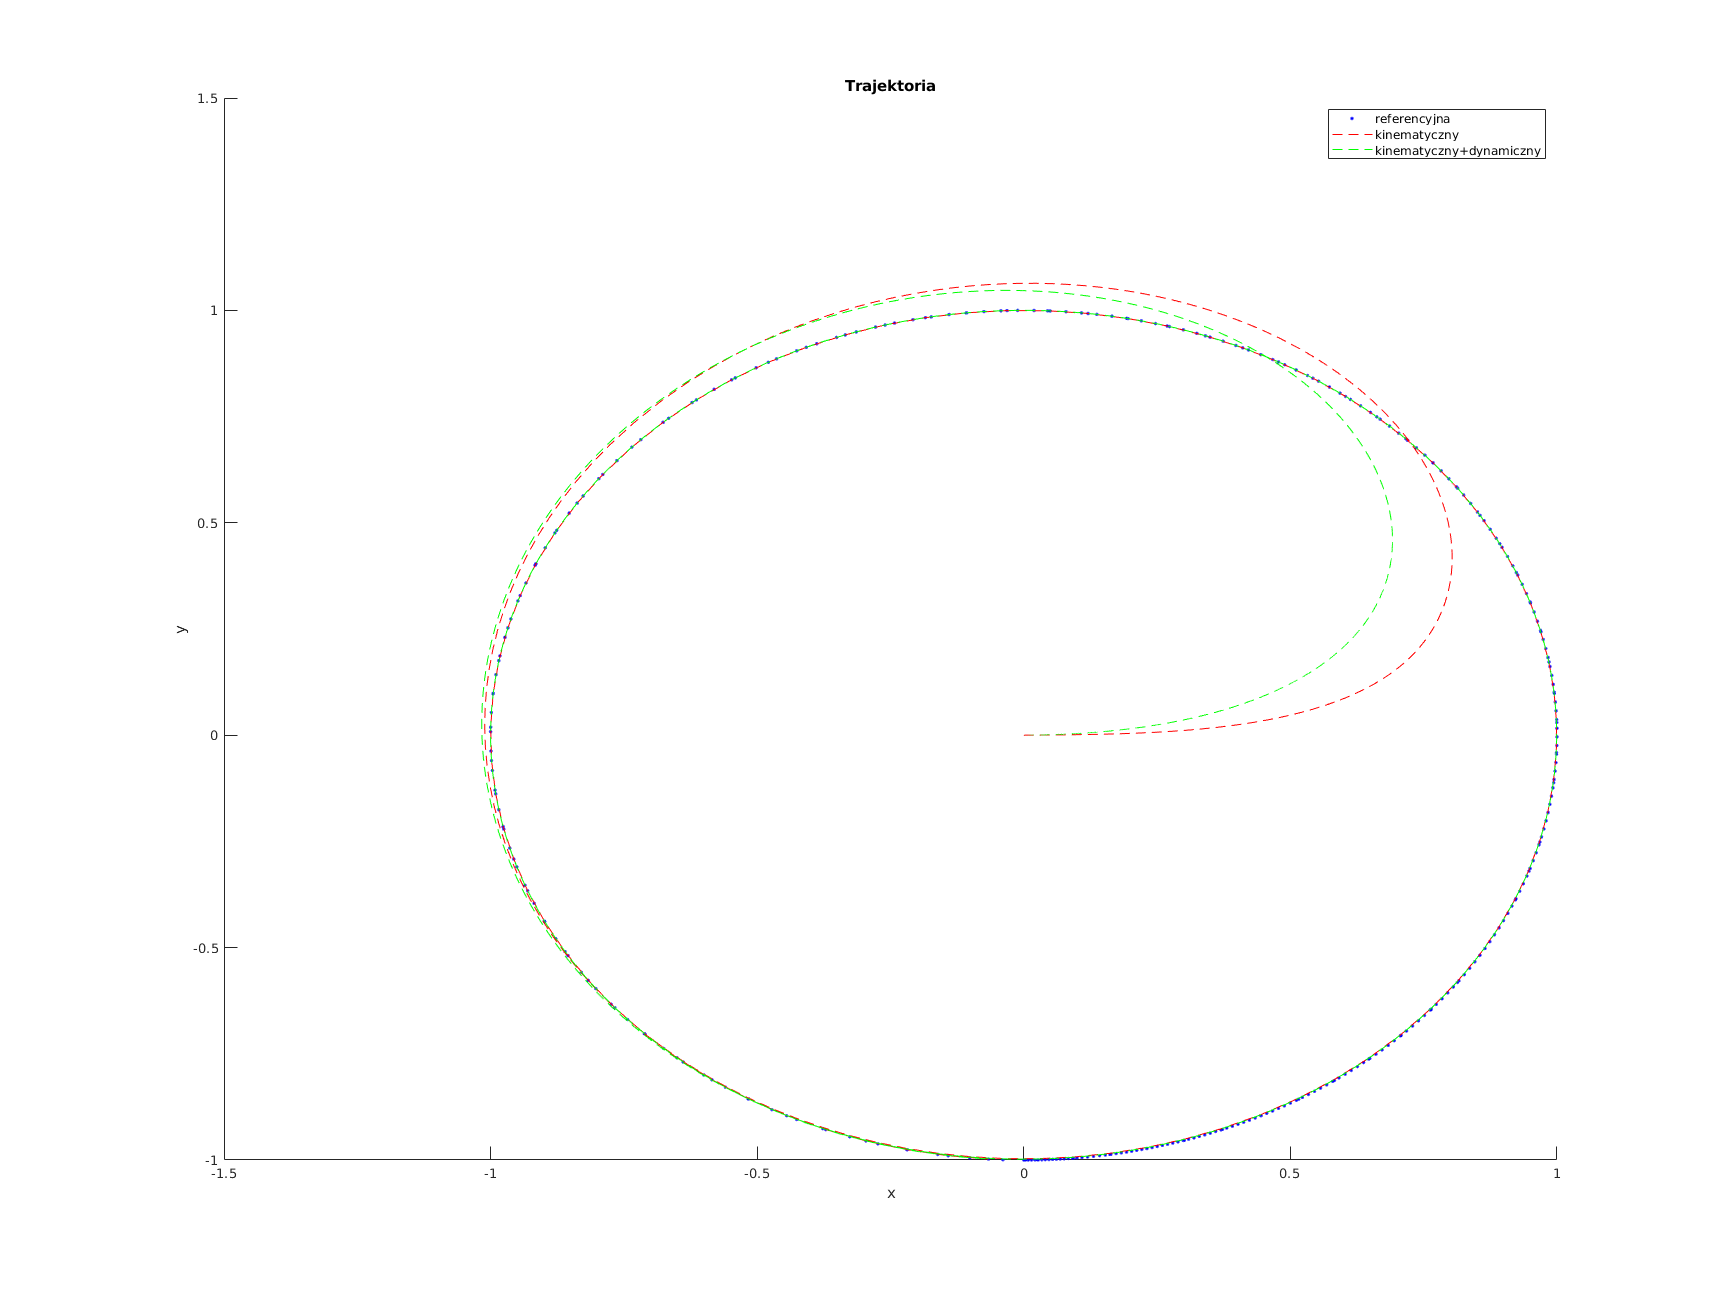
\includegraphics[width=1\textwidth]{figures/dyn_trajektoria.png}
      \caption{Trajektoria}
      \label{fig:4}
    \end{figure}

    Wykres \ref{fig:4} porównuje trajektorie referencyjną do trajektorii ze sterownikiem dynamicznym oraz bez sterownika dynamicznego. Dodanie sterowanika dynamicznego spowodowało bardziej zdecydowaną reakcję obiektu w początkowej fazie ruchu porównując z drugim mniej skomplikowanym rozwiązaniem. Jednakże czas potrzebny na osiągniecie zadanej trajektorii jest bardzo porównywalny. 

  \subsection{Zależność od współczynnika $K_1$}
  Wykres \ref{fig:5} przedstawia jak wpływa zmiana współczynnika $K_1$ na poszczególne błędy śledzenia, przy zachowaniu współczynników $K_2$ i $K_M$ równych 1. Na podstawie tych danych można wywnioskować że wzrost wzmocnienia $K_1$:

  \begin{itemize}
    \item znacznie zmniejsza błąd $E_x$ oraz skraca jego czas stabilizacji,
    \item powoduje mniej stromy spadek błędów $E_y$ oraz $E_\theta$ i wydłuża ich czas stabilizacji, niwelując przesterowania.
  \end{itemize}
  
  \begin{figure}[H]
    \centering
    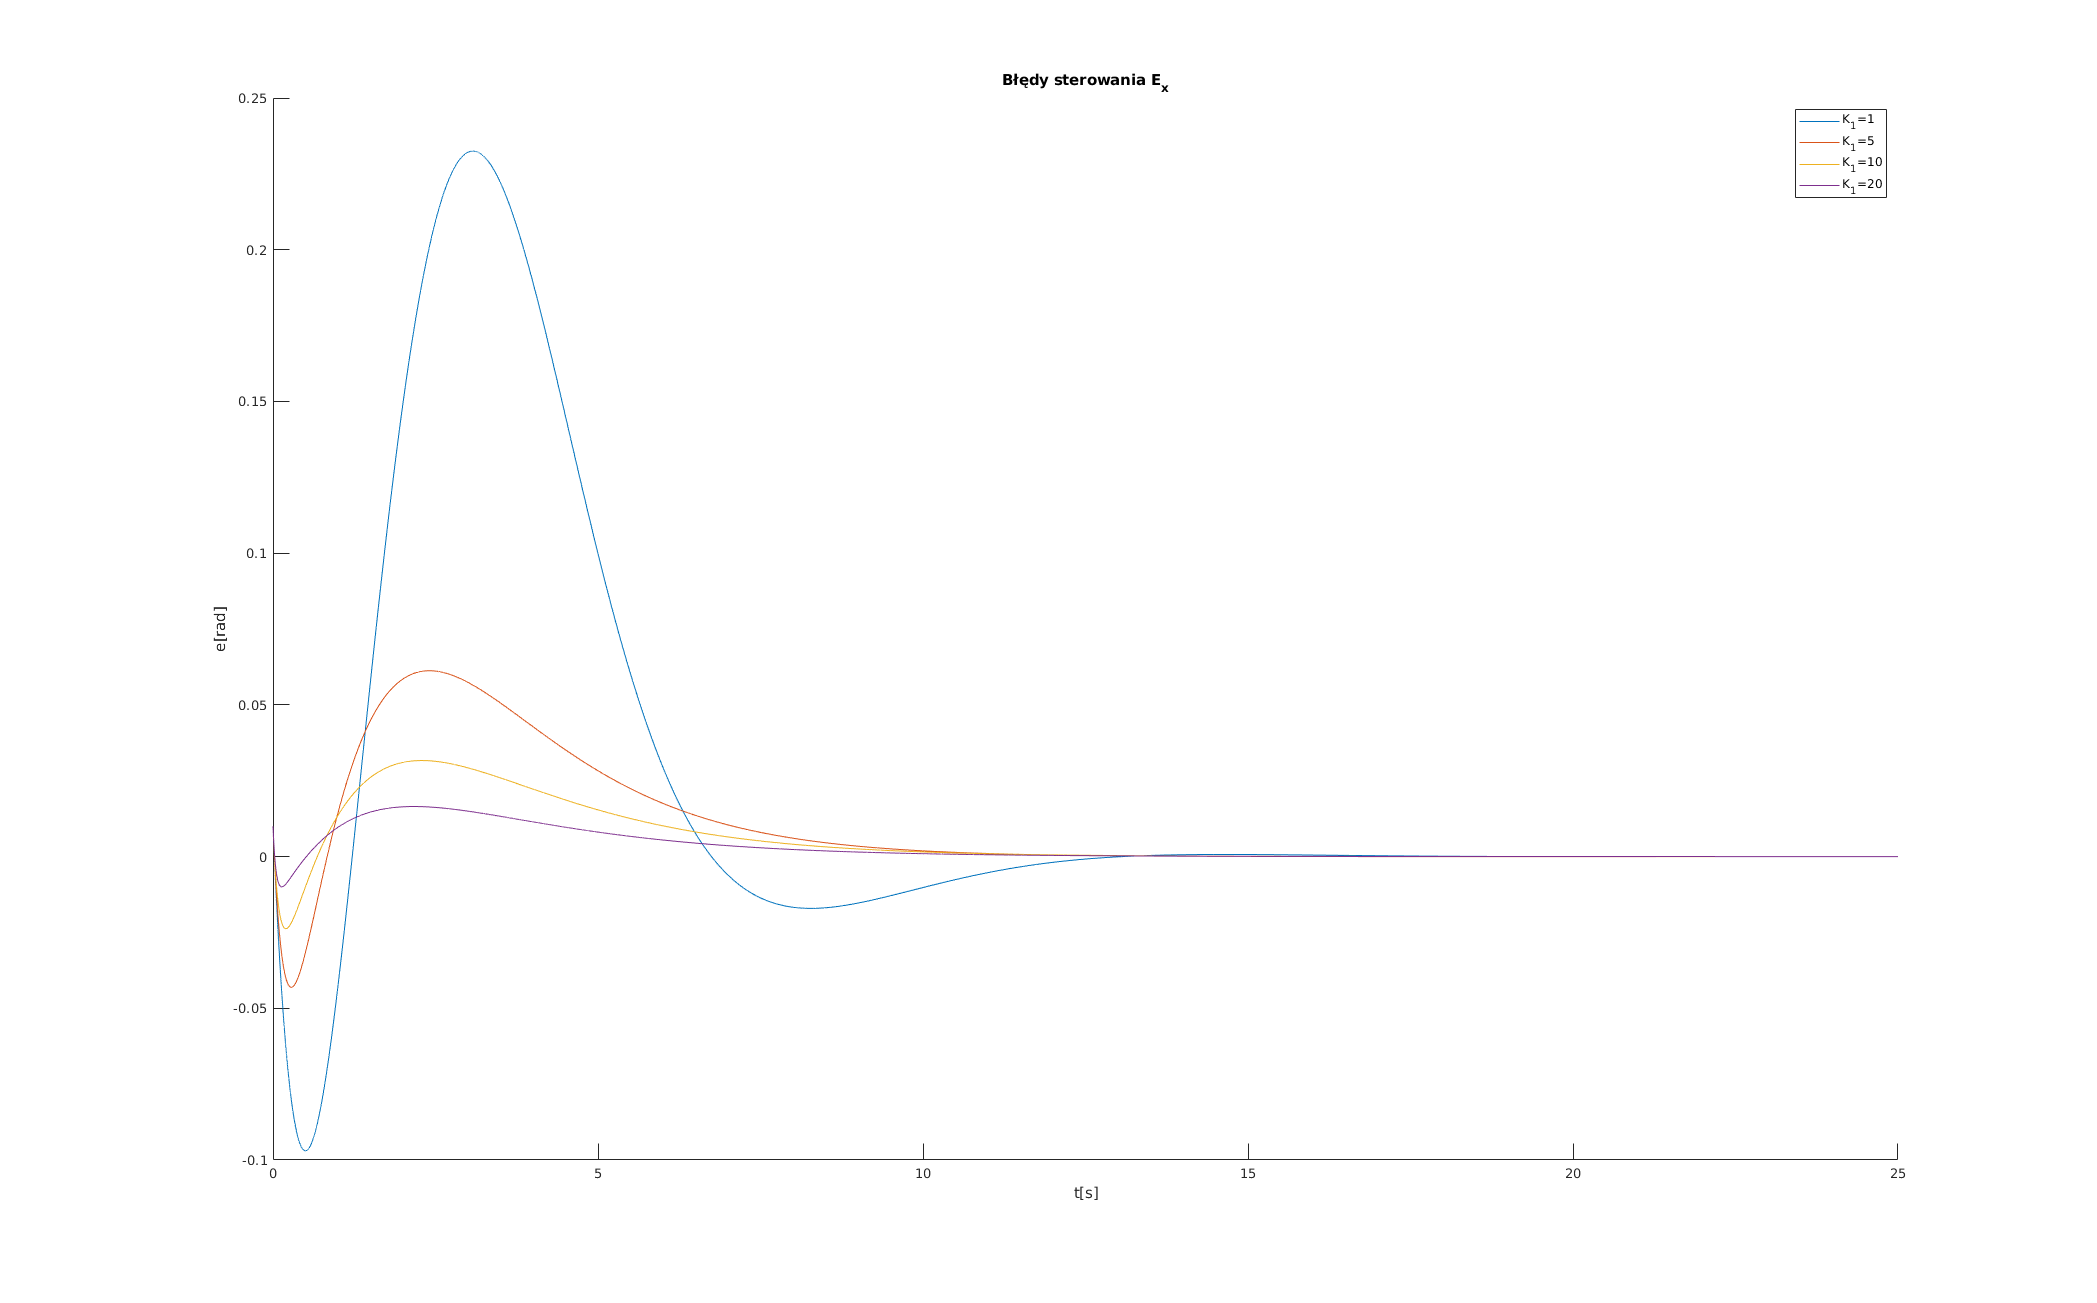
\includegraphics[height=0.33\textheight]{figures/dyn_bledy_k1_ex.png}
    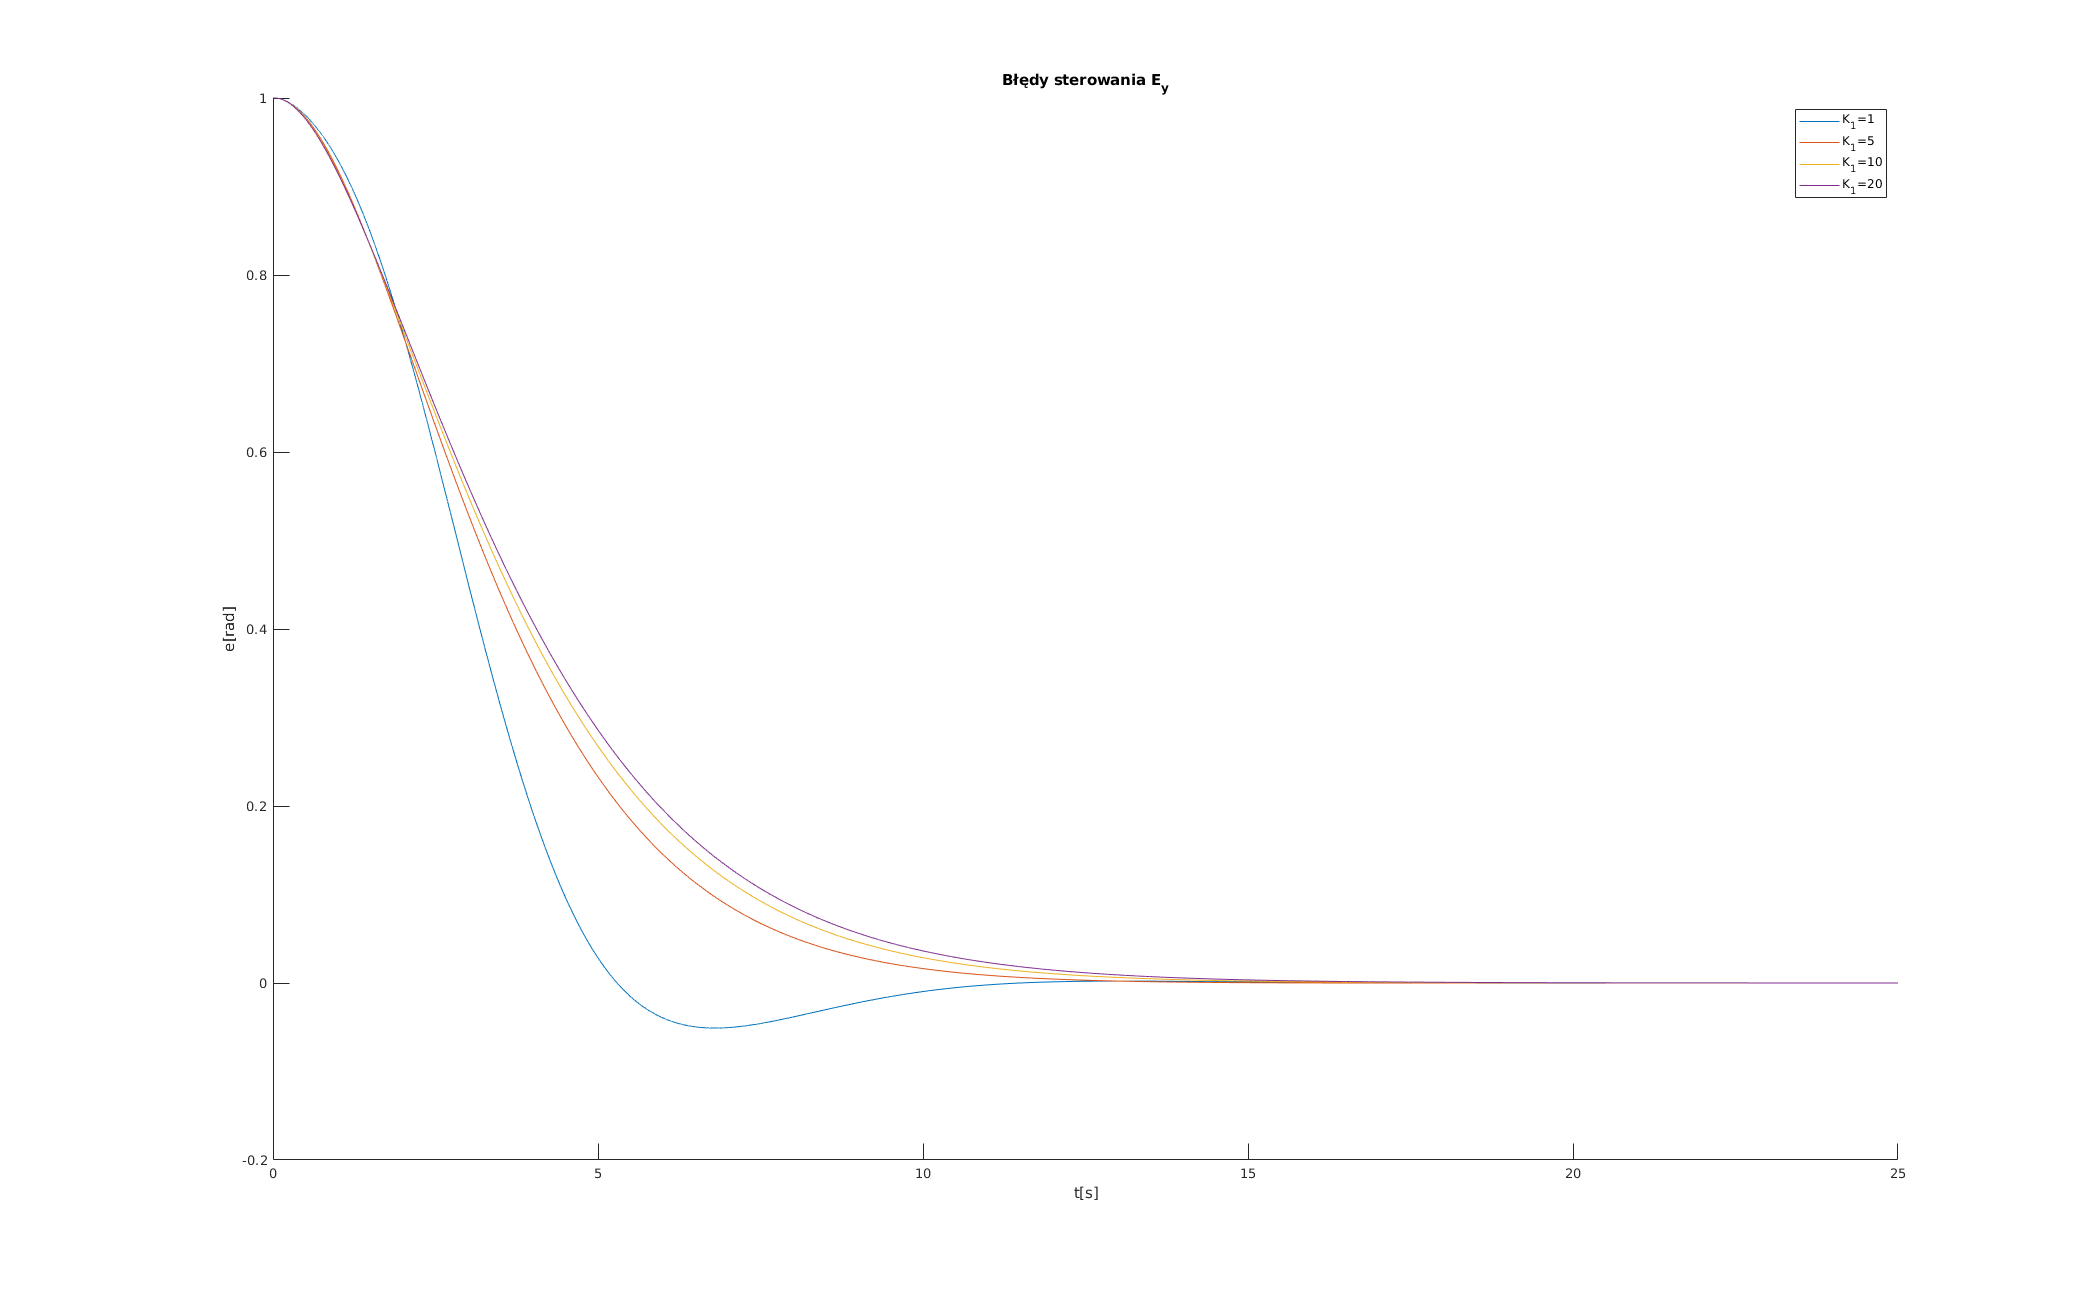
\includegraphics[height=0.33\textheight]{figures/dyn_bledy_k1_ey.png}
    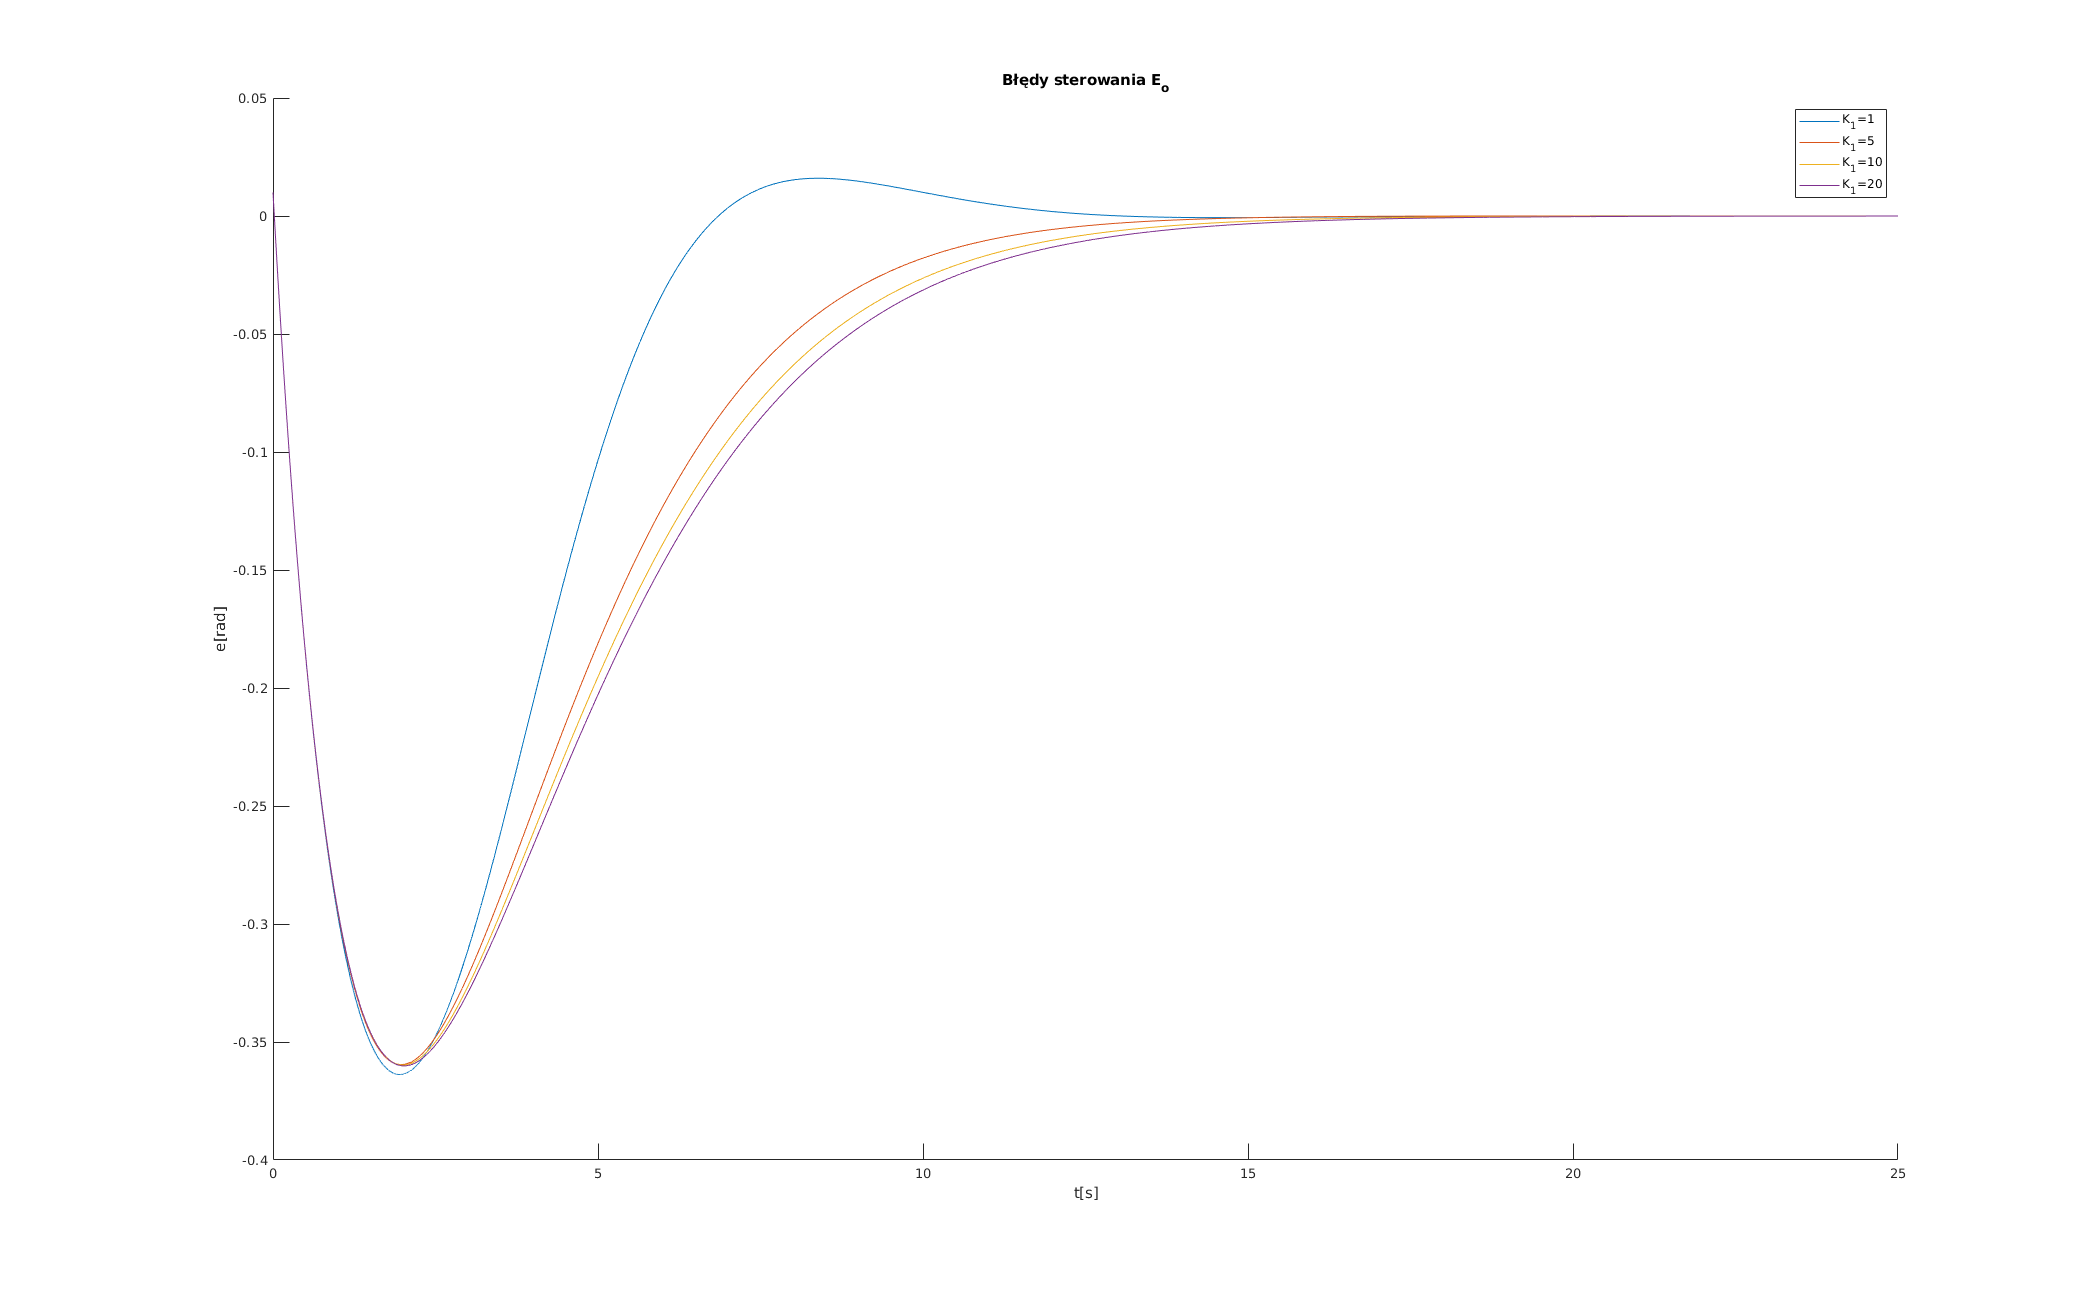
\includegraphics[height=0.33\textheight]{figures/dyn_bledy_k1_eo.png}
    \caption{Błędy $e_x$, $e_y$, $e_\theta$}
    \label{fig:5}
  \end{figure}

  \begin{figure}[H]
    \centering
    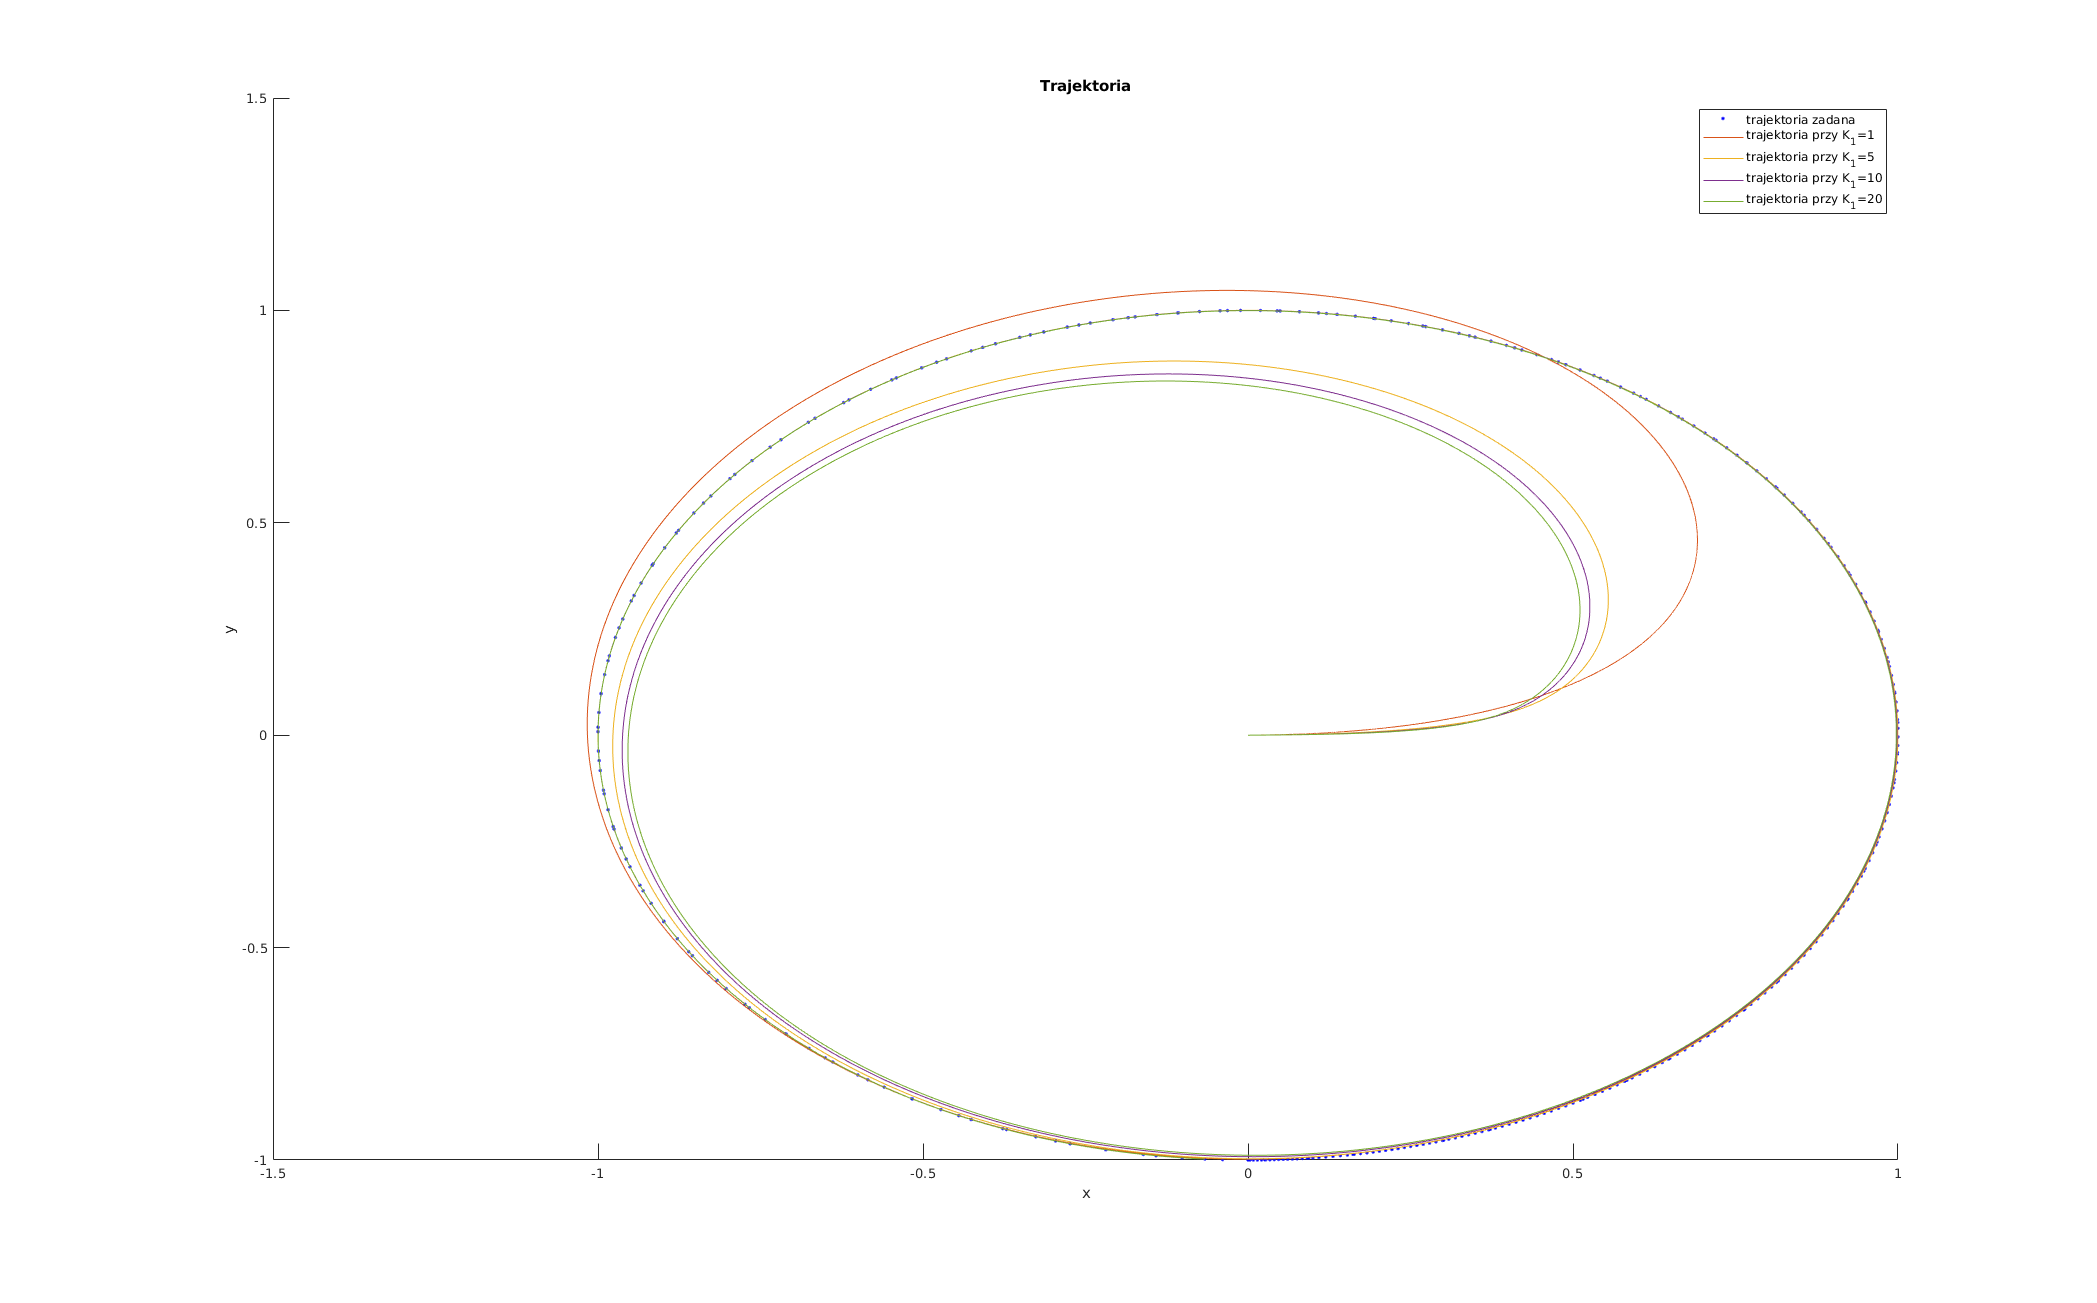
\includegraphics[width=1\textwidth]{figures/dyn_trajektoria_k1.png}
    \caption{Trajektorie zależne od $K_1$}
    \label{fig:6}
  \end{figure}


  \subsection{Zależność od współczynnika $K_2$}
  Wykres \ref{fig:7} przedstawia jak wpływa zmiana współczynnika $K_2$ na poszczególne błędy śledzenia, przy zachowaniu współczynników $K_1$ i $K_M$ równych 1. Na podstawie tych danych można wywnioskować że wzrost wzmocnienia $K_2$:

  \begin{itemize}
    \item znacznie zmniejsza błąd $E_\theta$ oraz skraca jego czas stabilizacji,
    \item powoduje mniej stromy spadek błędów $E_x$ oraz $E_y$ i wydłuża ich czas stabilizacji, niwelując przesterowania.
  \end{itemize}
  
  \begin{figure}[H]
    \centering
    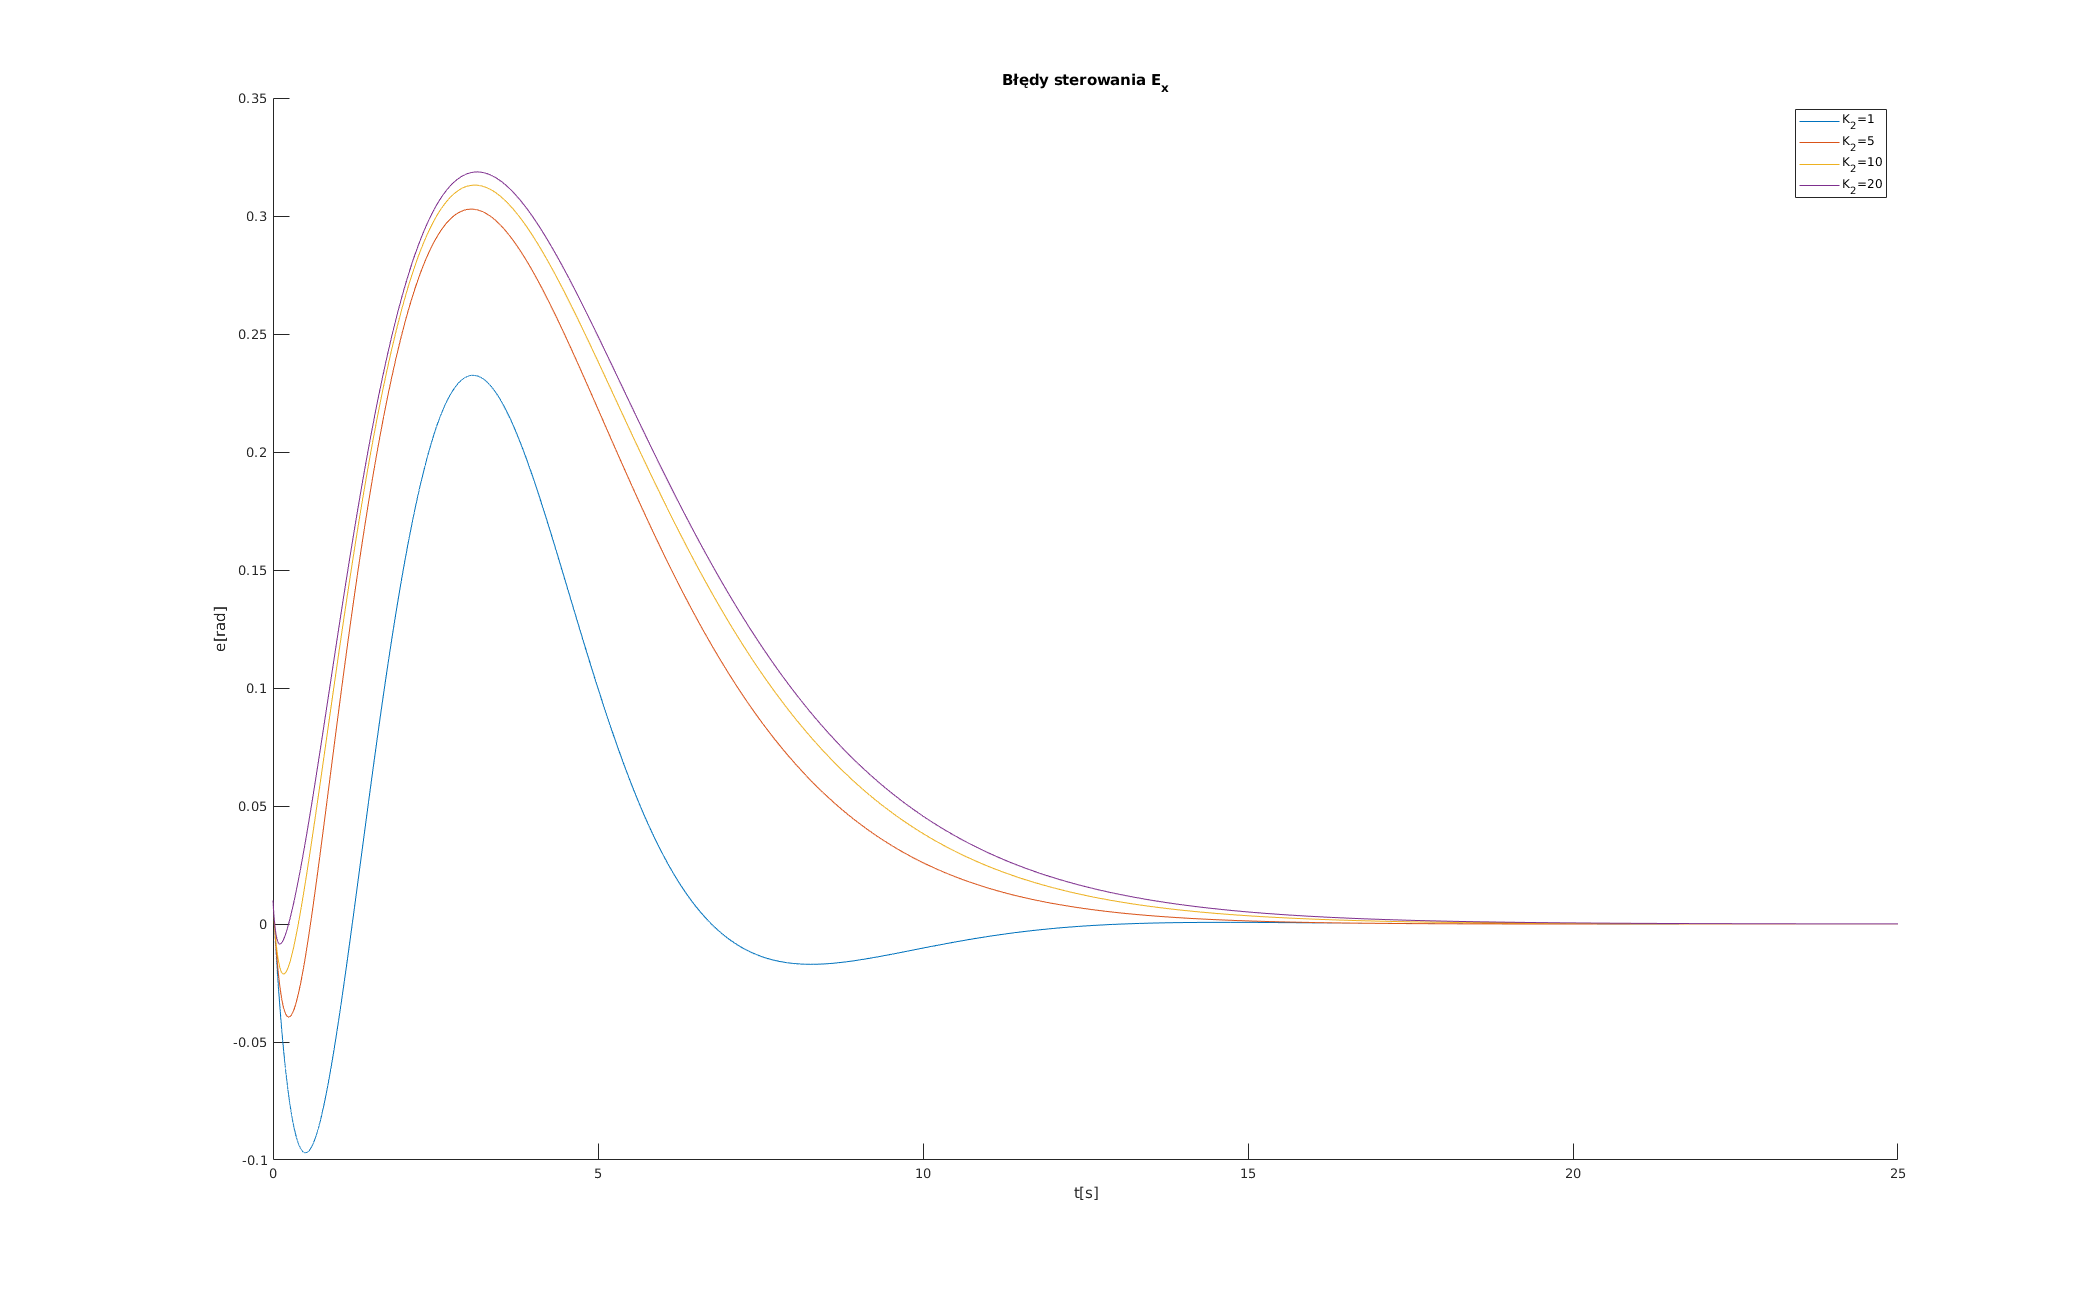
\includegraphics[height=0.33\textheight]{figures/dyn_bledy_k2_ex.png}
    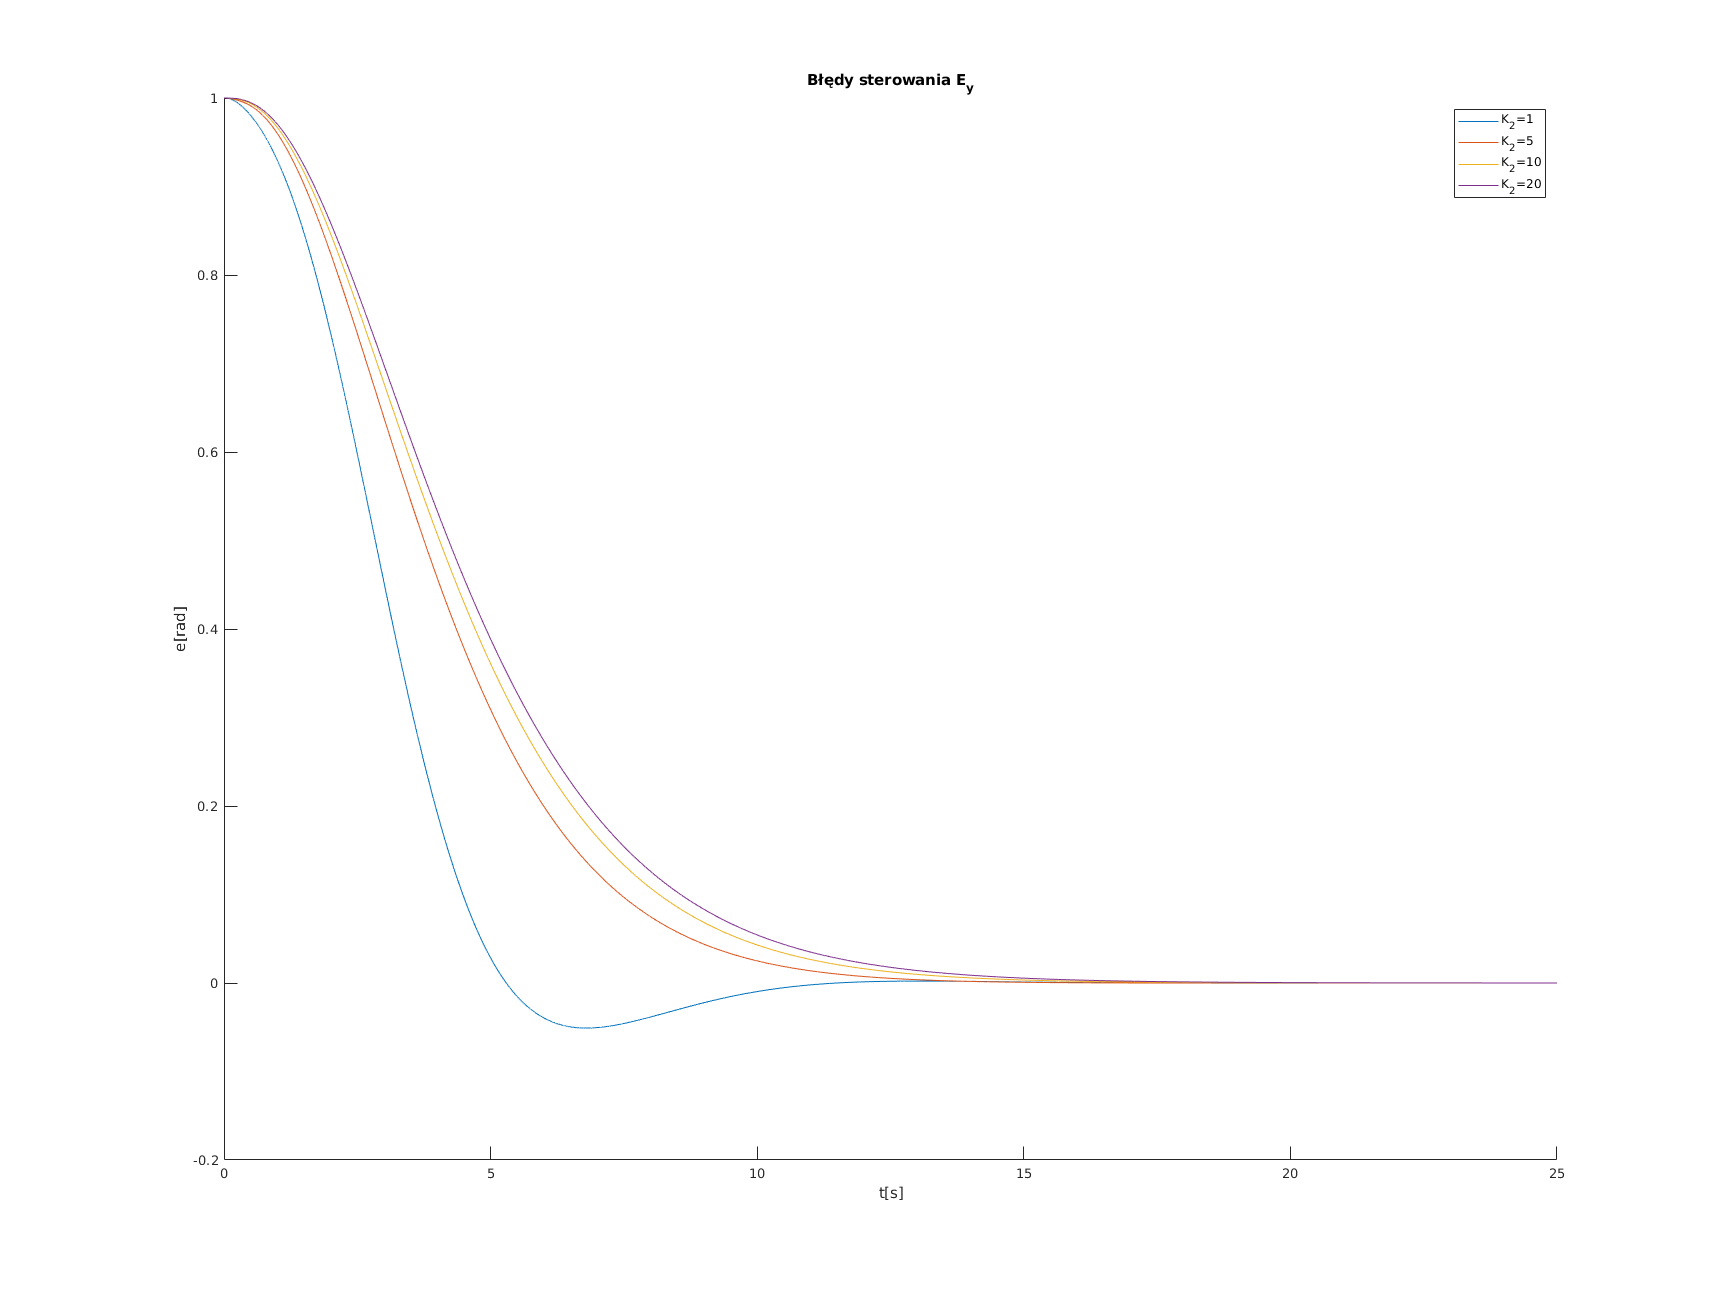
\includegraphics[height=0.33\textheight]{figures/dyn_bledy_k2_ey.png}
    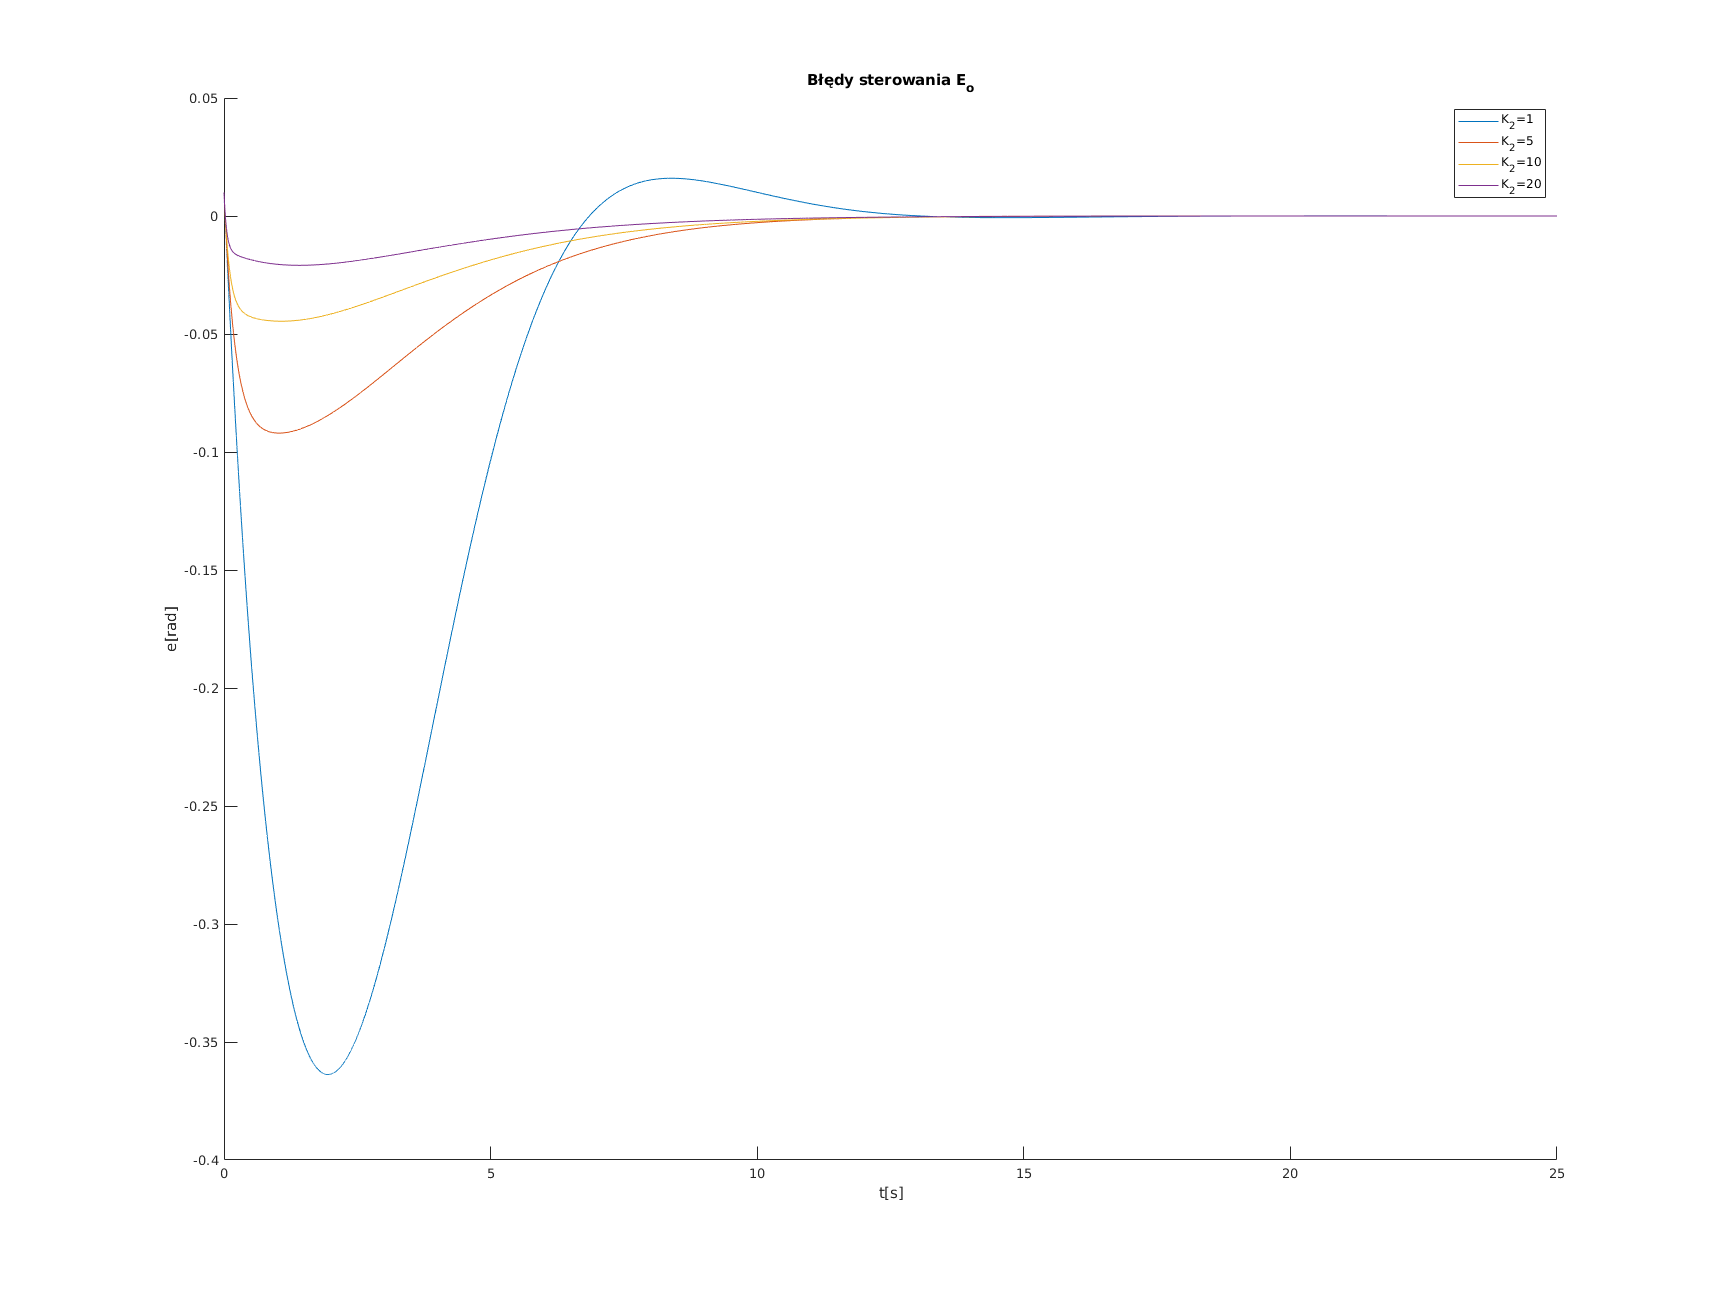
\includegraphics[height=0.33\textheight]{figures/dyn_bledy_k2_eo.png}
    \caption{Błędy $e_x$, $e_y$, $e_\theta$}
    \label{fig:7}
  \end{figure}

  \begin{figure}[H]
    \centering
    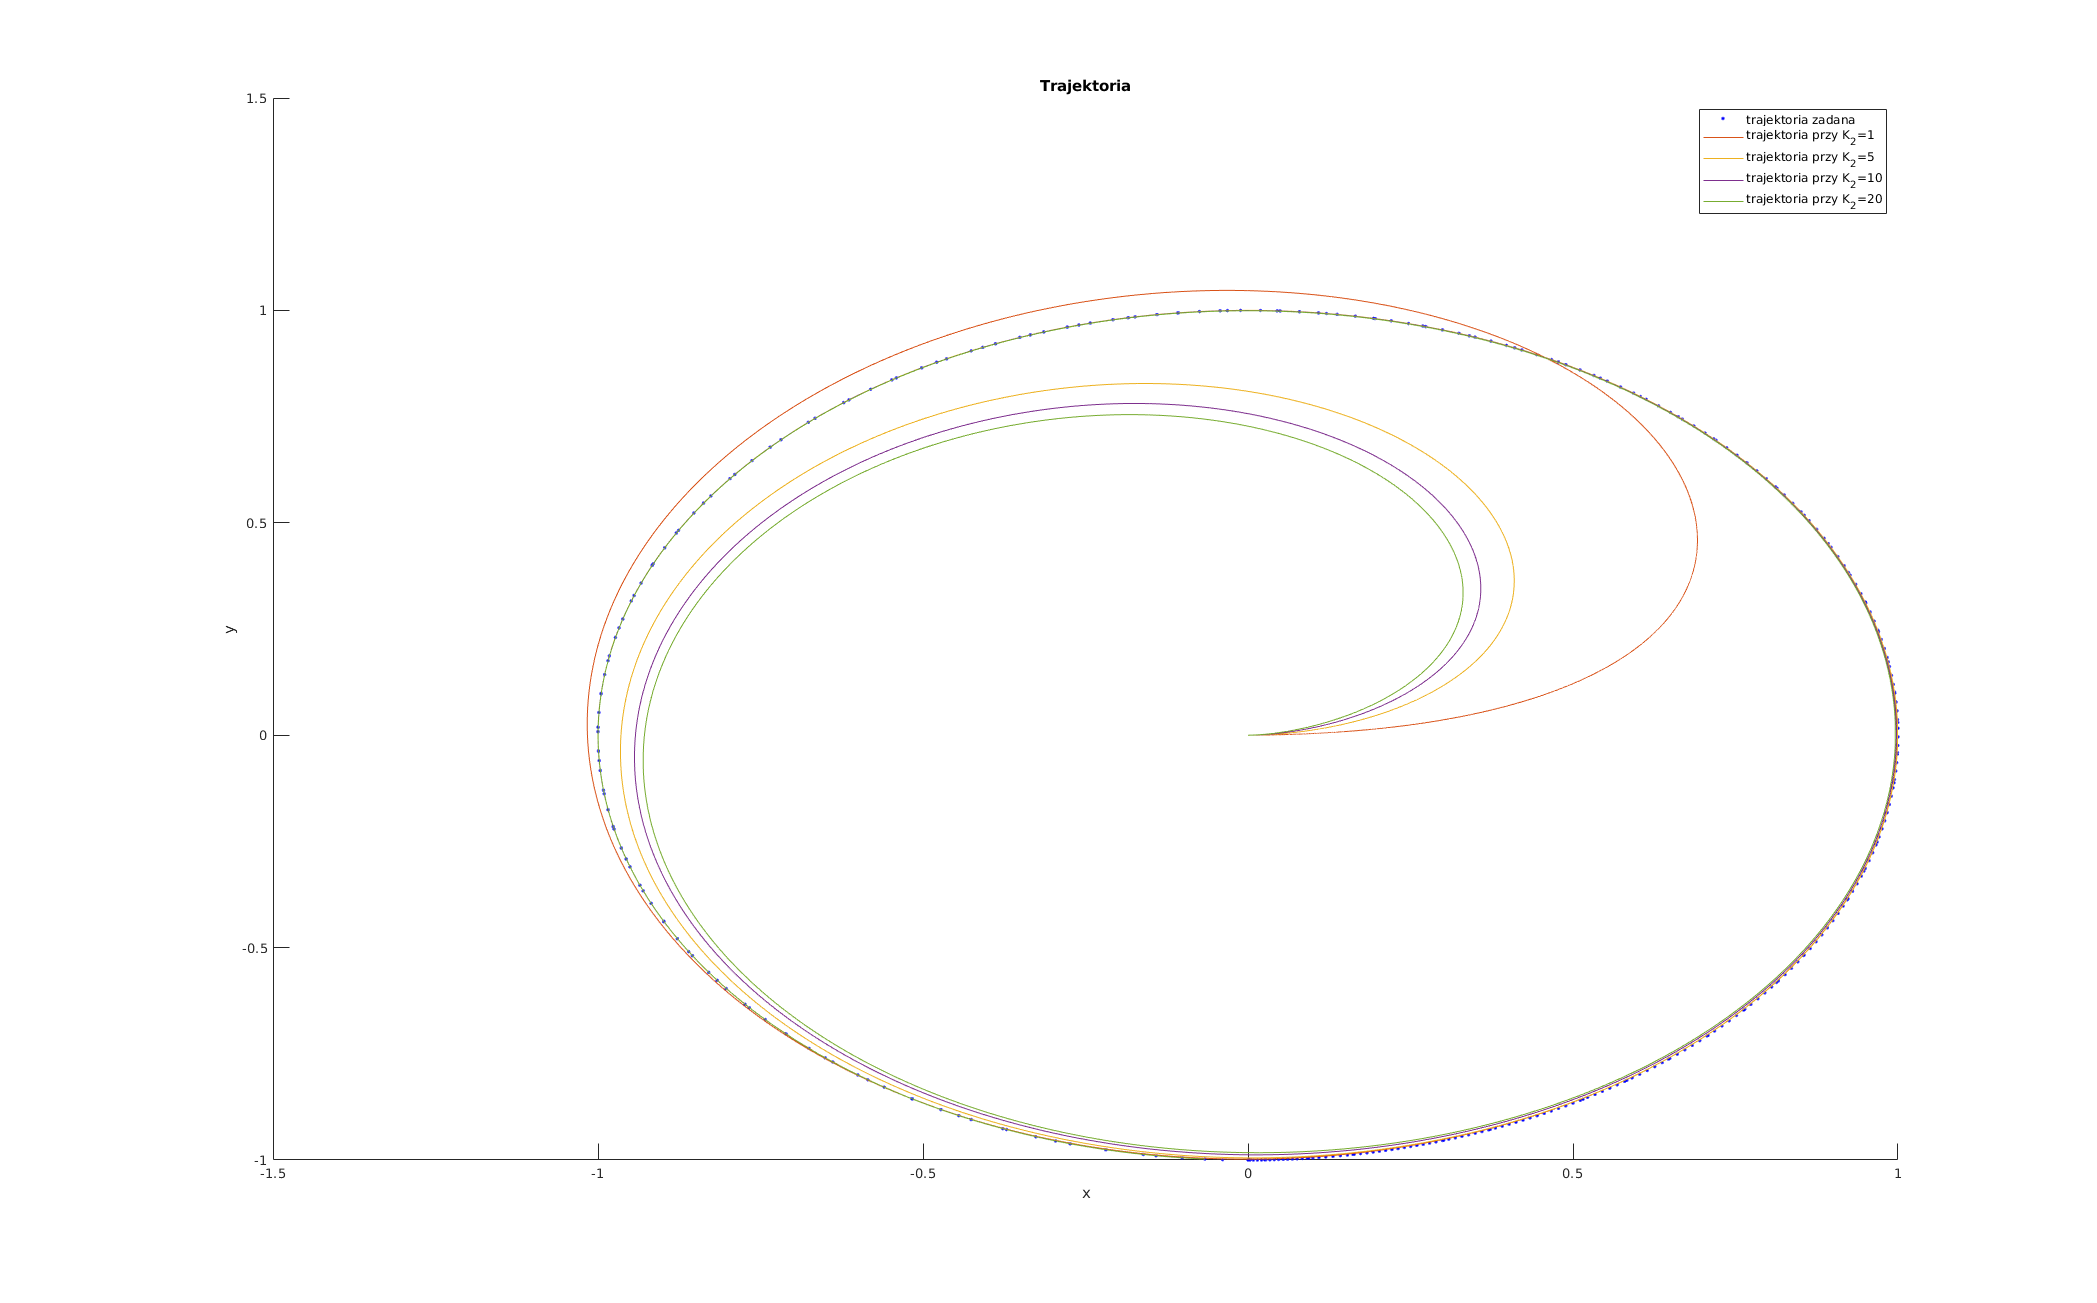
\includegraphics[width=1\textwidth]{figures/dyn_trajektoria_k2.png}
    \caption{Trajektorie zależne od $K_2$}
    \label{fig:8}
  \end{figure}


  \subsection{Zależność od współczynnika $K_M$}
  Wykres \ref{fig:9} przedstawia jak wpływa zmiana współczynnika $K_M$ na poszczególne błędy śledzenia, przy zachowaniu współczynników $K_1$ i $K_2$ równych 1. Na podstawie tych danych można wywnioskować że wzrost wzmocnienia $K_M$:

  \begin{itemize}
    \item przyśpiesza reakcję sterownika oraz zwiększa błąd $E_x$,
    \item nieznacznie przyśpiesza reakcję sterownika oraz zwiększa błędy $E_y$ i $E_\theta$,
  \end{itemize}
  
  \begin{figure}[H]
    \centering
    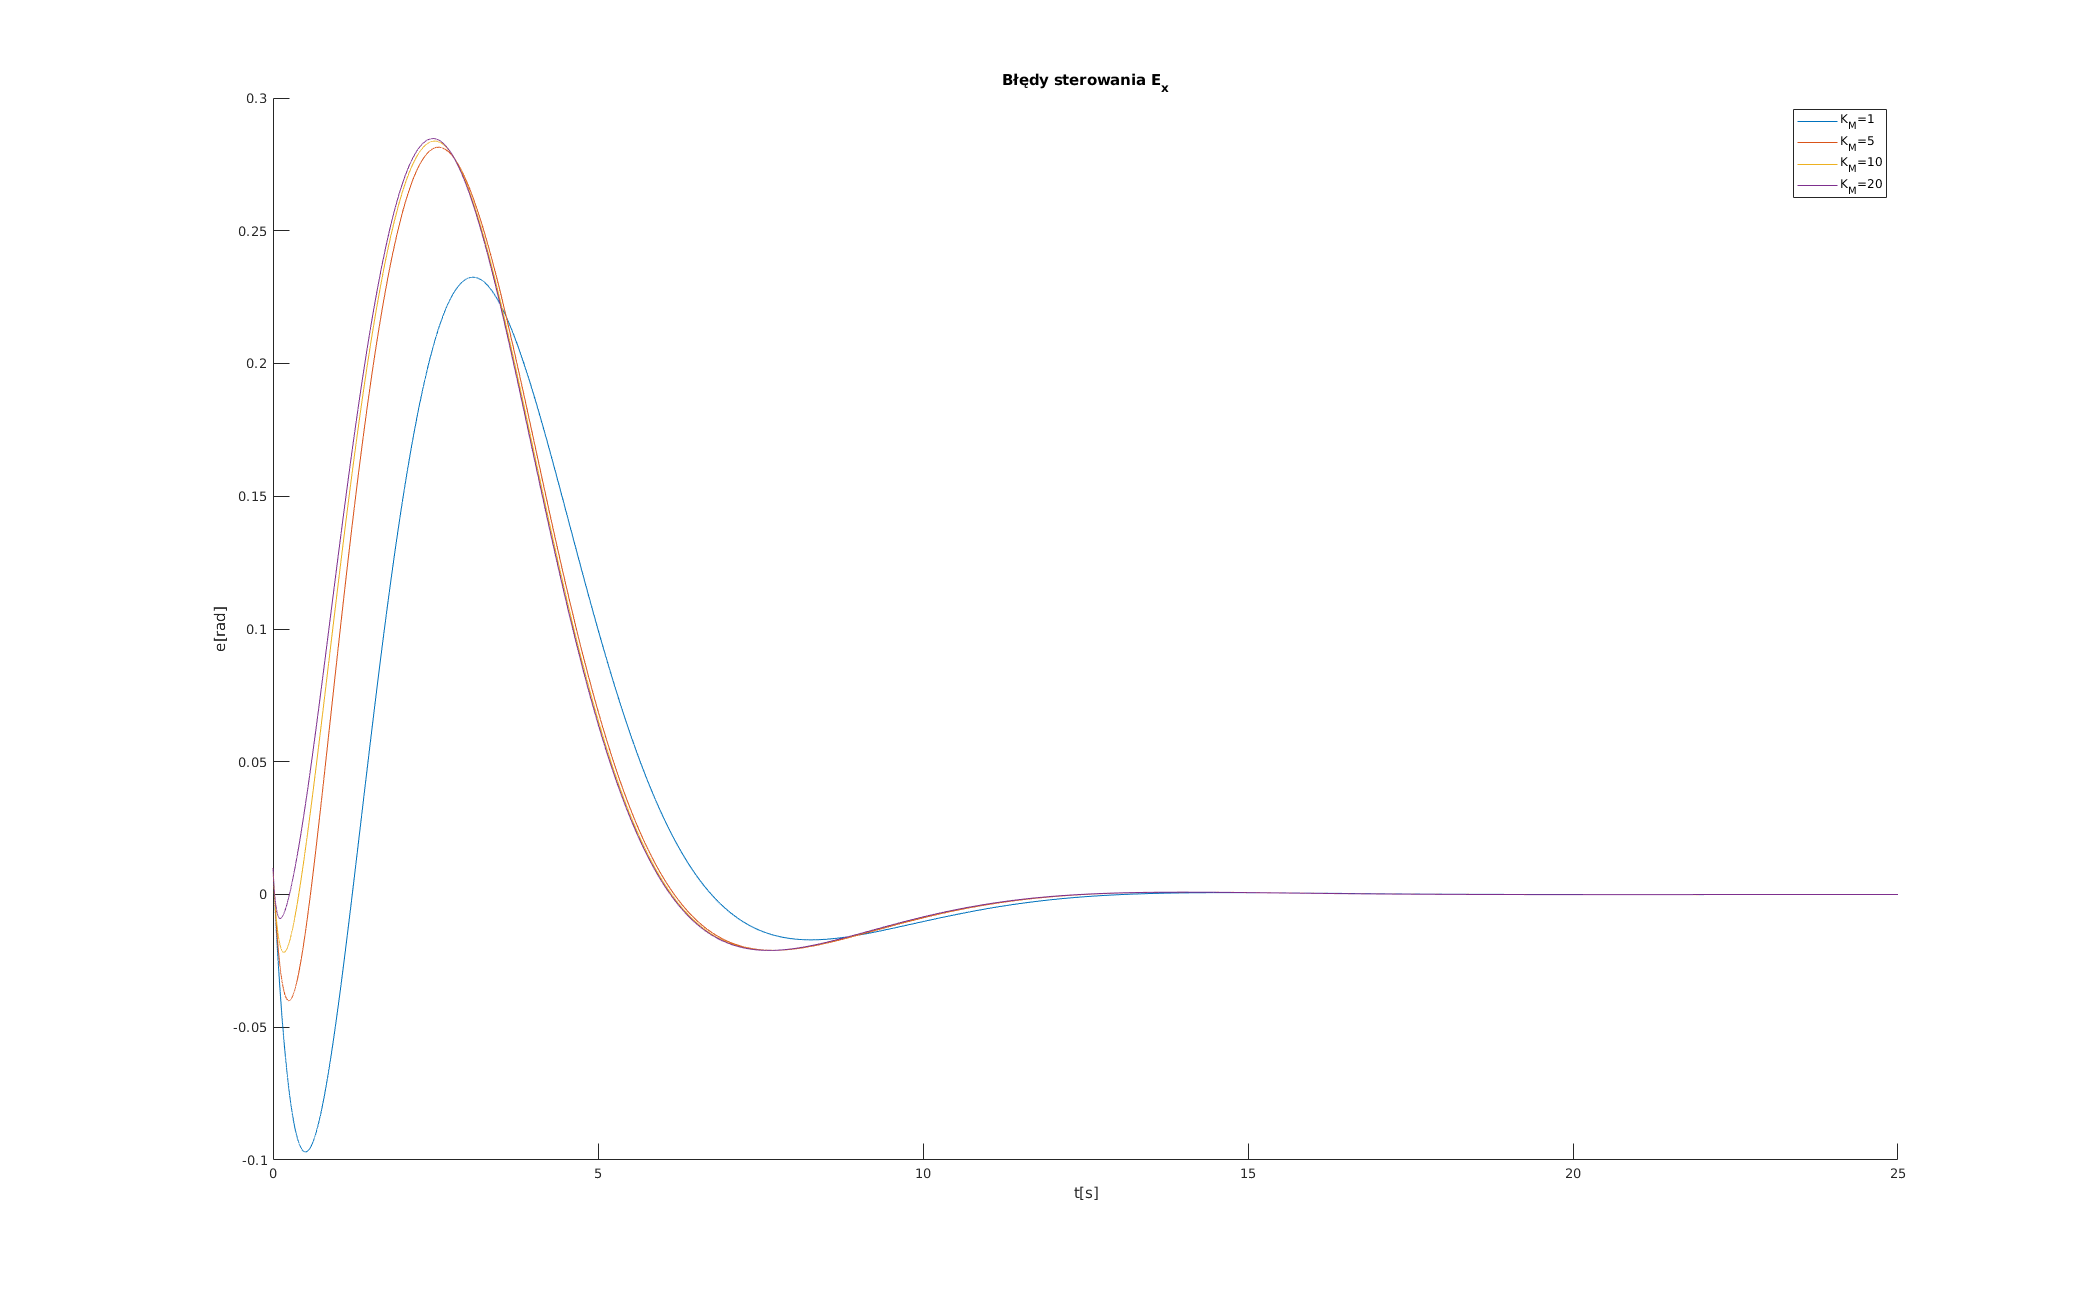
\includegraphics[height=0.33\textheight]{figures/dyn_bledy_km_ex.png}
    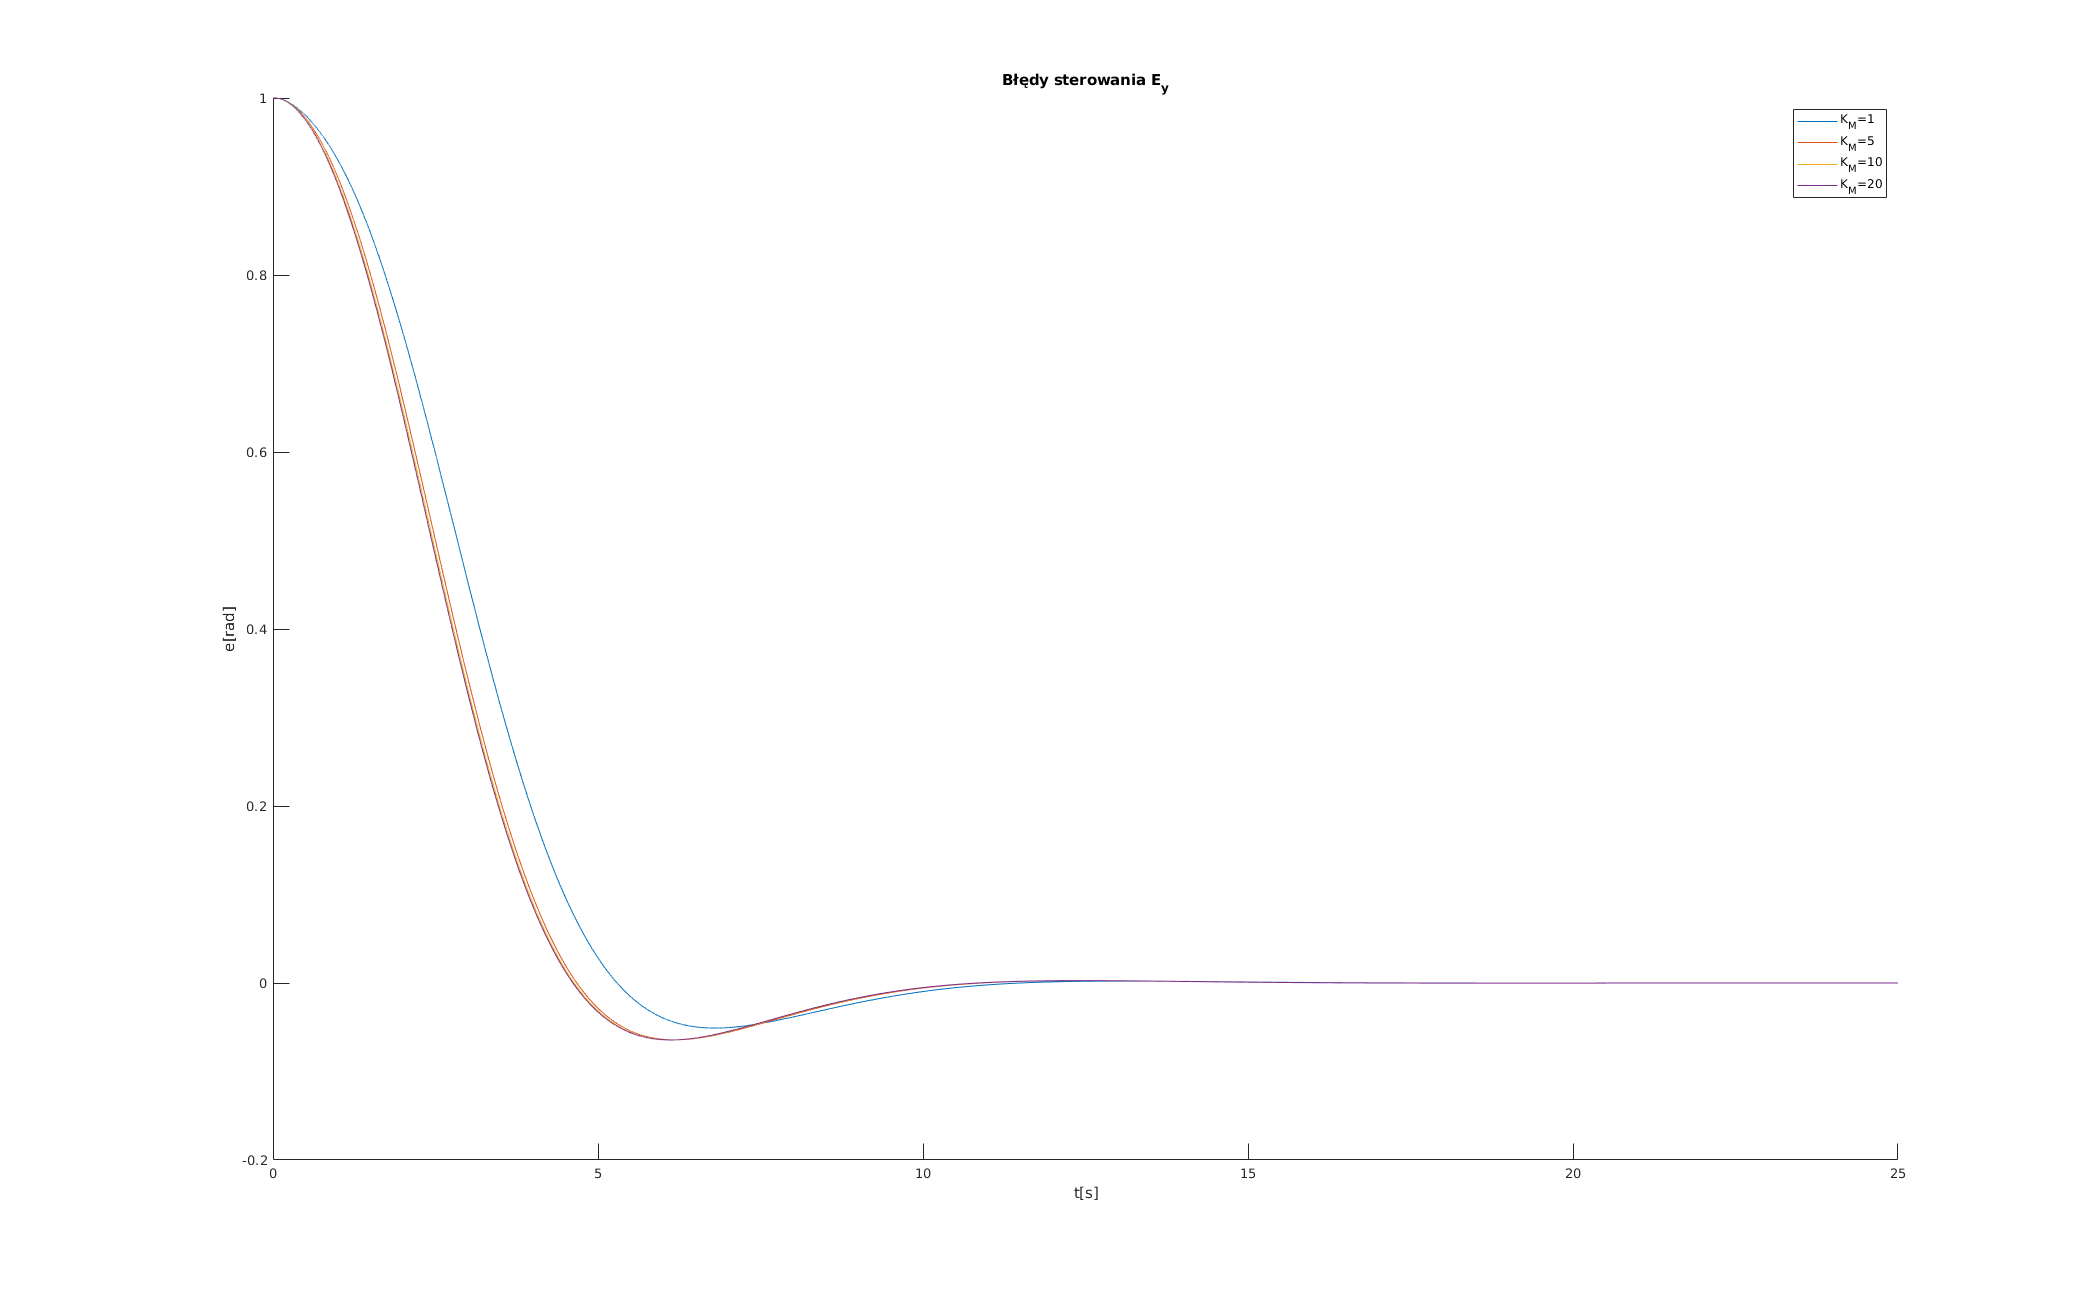
\includegraphics[height=0.33\textheight]{figures/dyn_bledy_km_ey.png}
    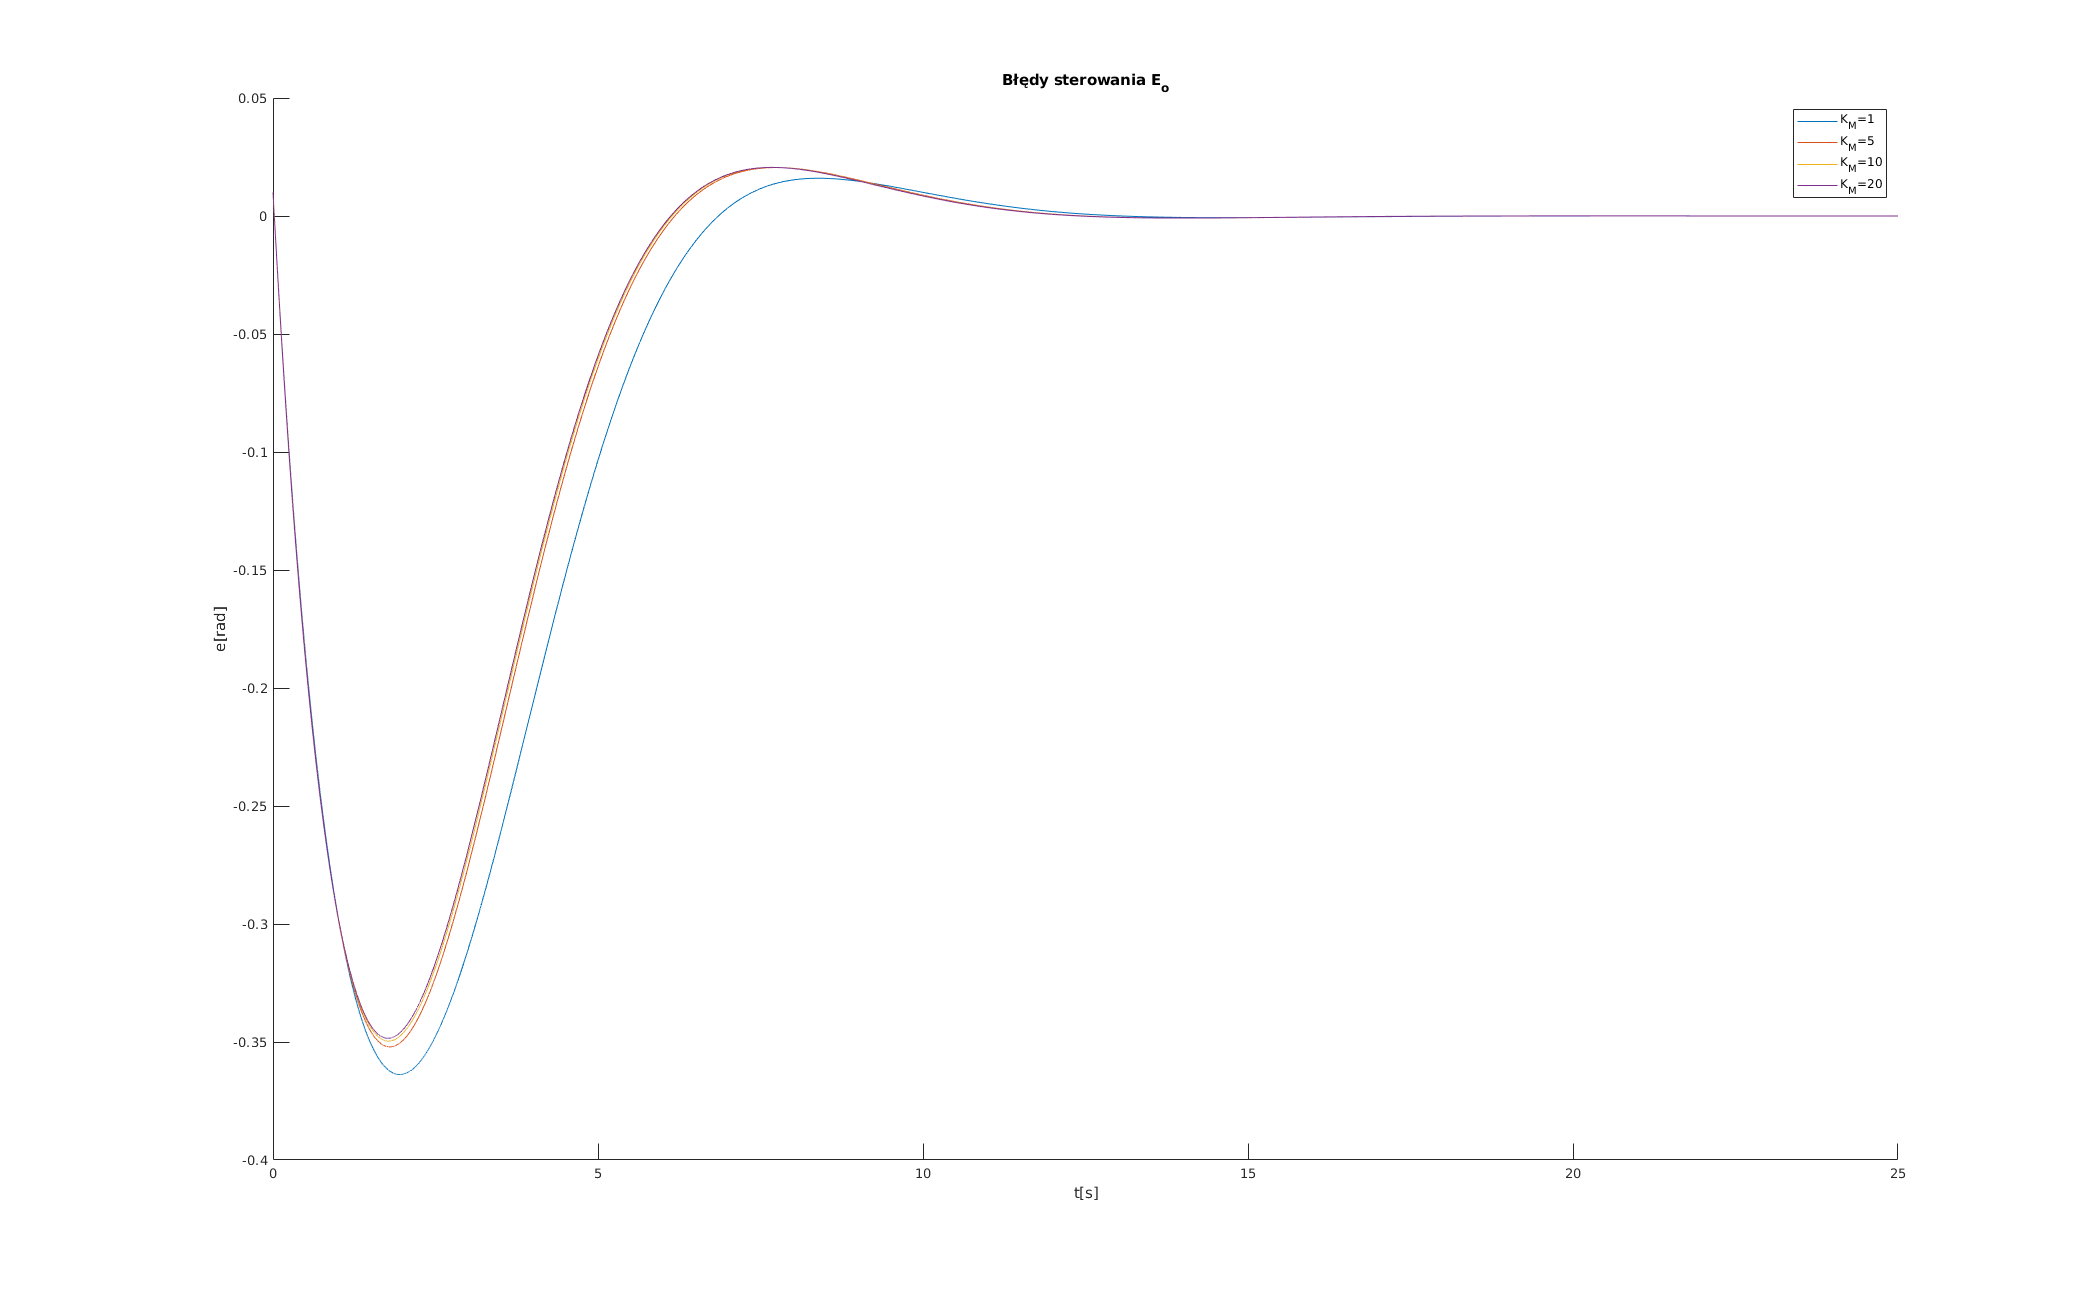
\includegraphics[height=0.33\textheight]{figures/dyn_bledy_km_eo.png}
    \caption{Błędy $e_x$, $e_y$, $e_\theta$}
    \label{fig:9}
  \end{figure}


  \begin{figure}[H]
    \centering
    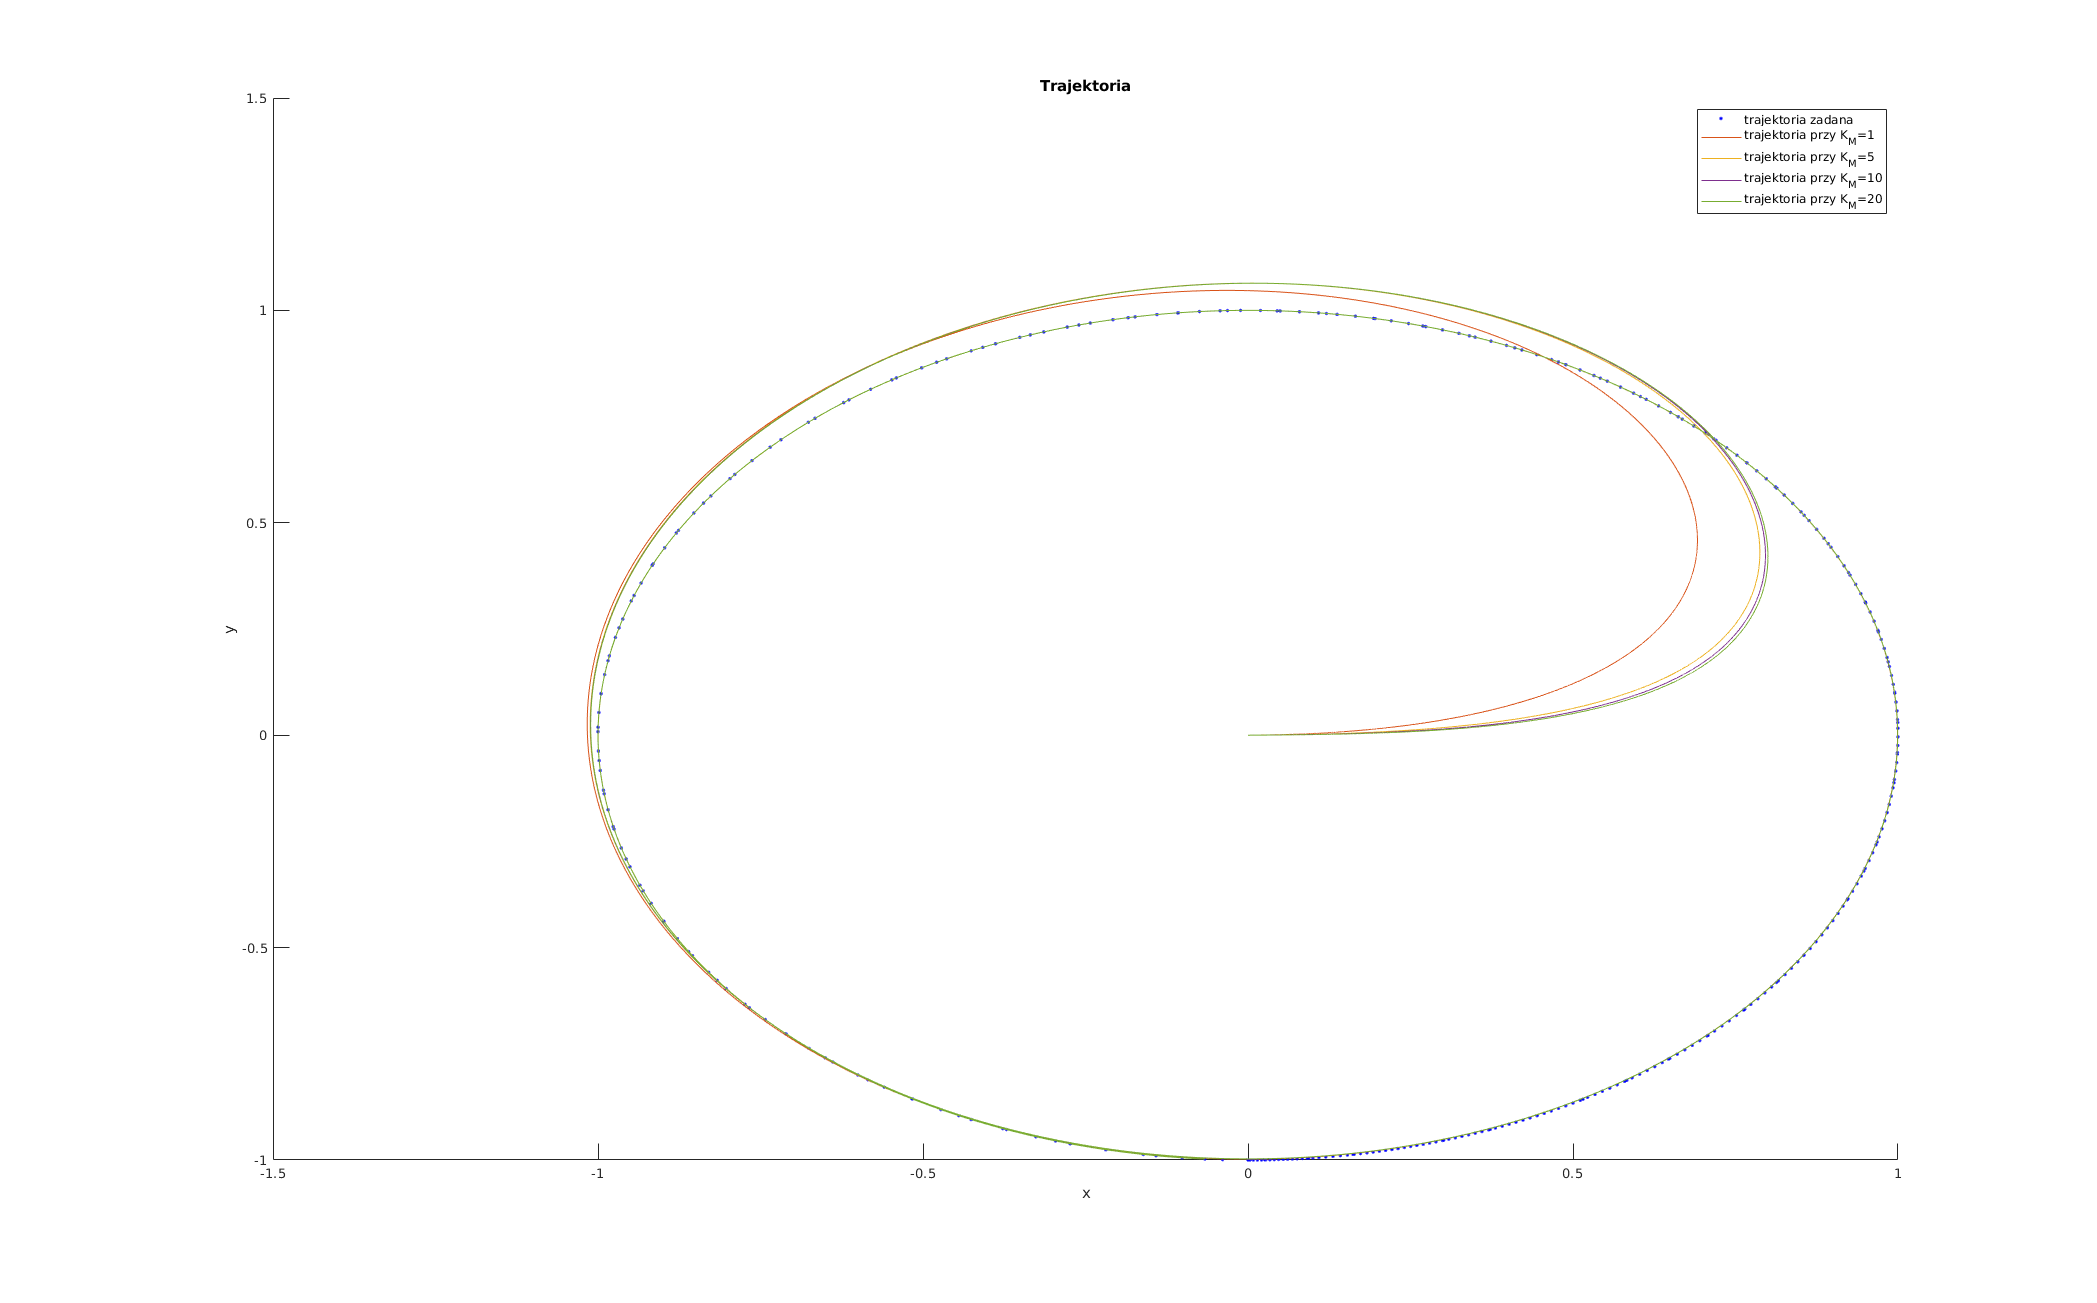
\includegraphics[width=1\textwidth]{figures/dyn_trajektoria_km.png}
    \caption{Trajektorie zależne od $K_M$}
    \label{fig:10}
  \end{figure}



  \subsection{Zależność od warunków początkowych}
  Zmiana warunków początkowych pozwala na zmianę miejsca startu algorytmu. Zmiana $x_0$ wpływa na pozycję na osi OX na trajektorii (patrz wykres \ref{fig:11}). W podobny sposób wpływa zmiana $y_0$ na pozycję na osi OY (patrz wykres \ref{fig:12}). Ostatni warunkiem początkowym jest $\theta_0$ wpływający na kąt ustawienia platformy. Warto zaznaczyć że nie wszystkie ustawienia kąta będą poprawne co można zaobserwować na wykresie \ref{fig:13}.

  \begin{figure}[H]
    \centering
    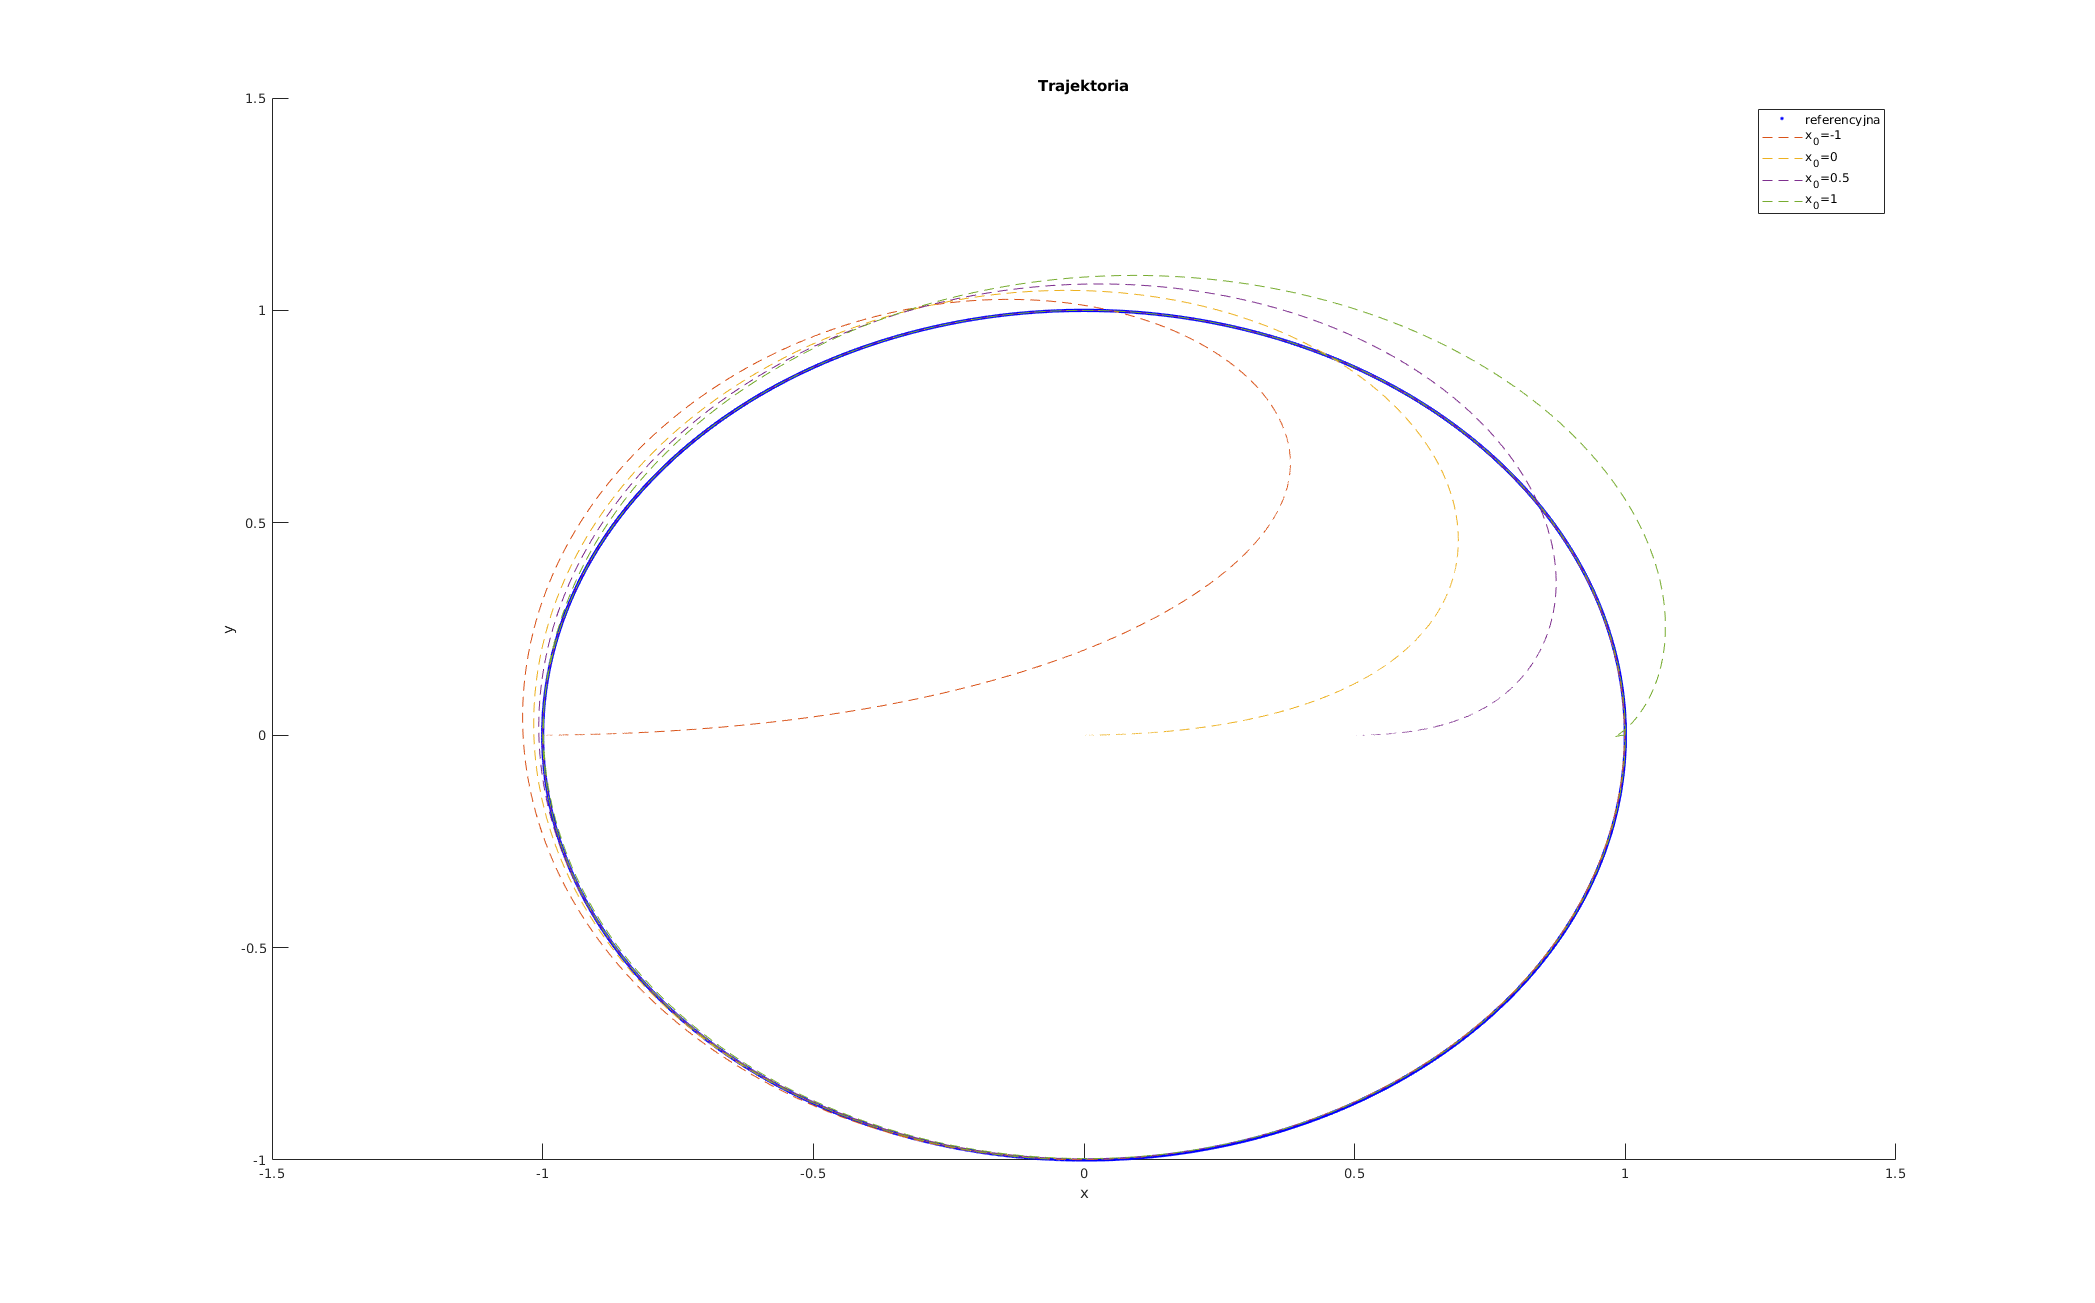
\includegraphics[width=1\textwidth]{figures/wp_x.png}
    \caption{Trajektorie zależne od $x_0$}
    \label{fig:11}
  \end{figure}

  \begin{figure}[H]
    \centering
    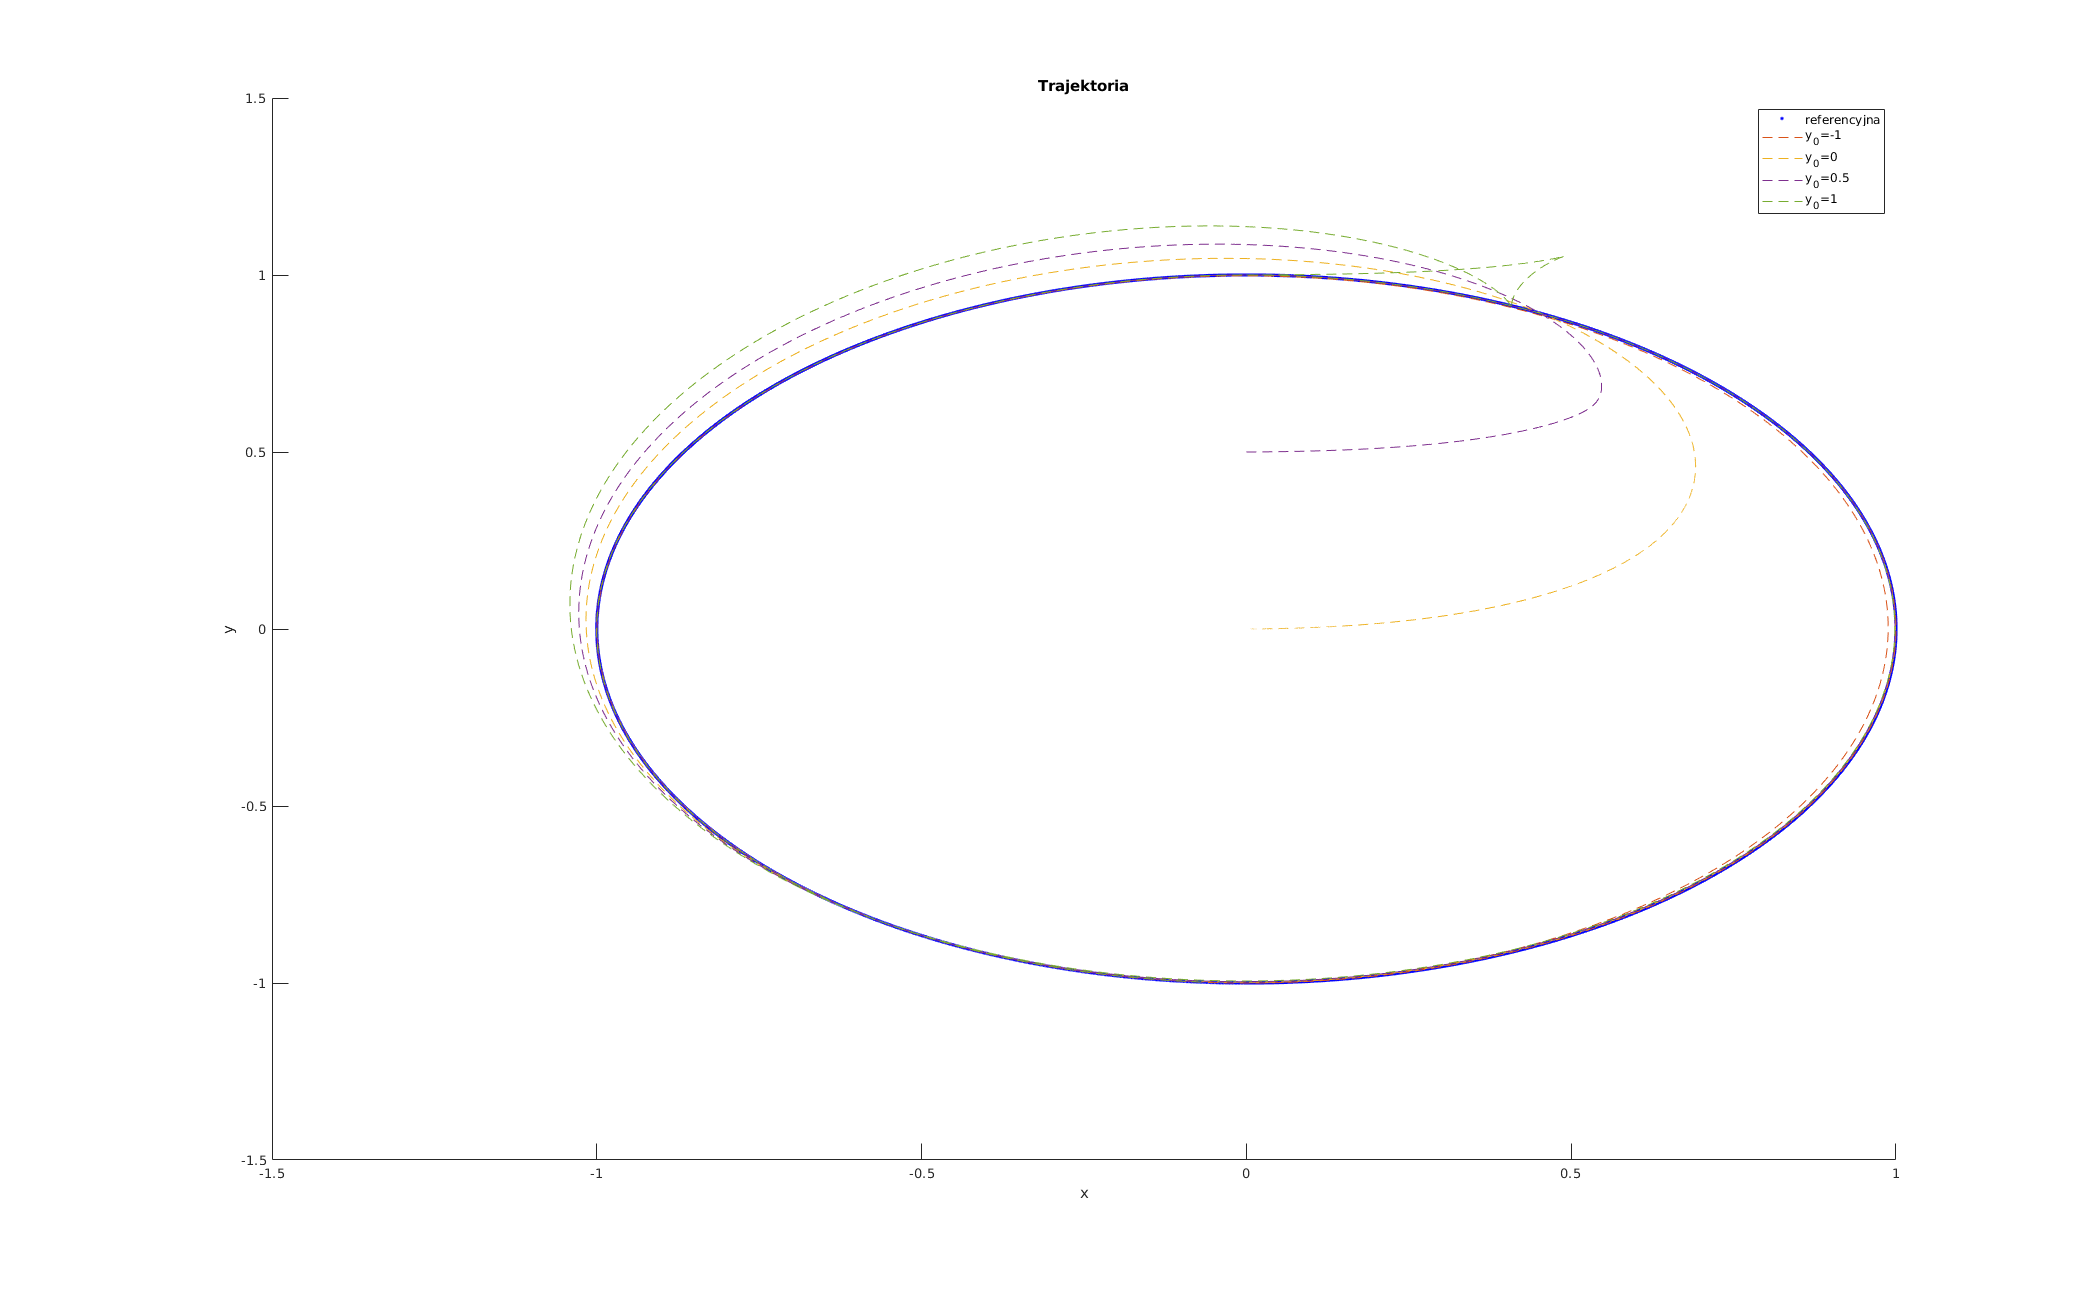
\includegraphics[width=1\textwidth]{figures/wp_y.png}
    \caption{Trajektorie zależne od $y_0$}
    \label{fig:12}
  \end{figure}

  \begin{figure}[H]
    \centering
    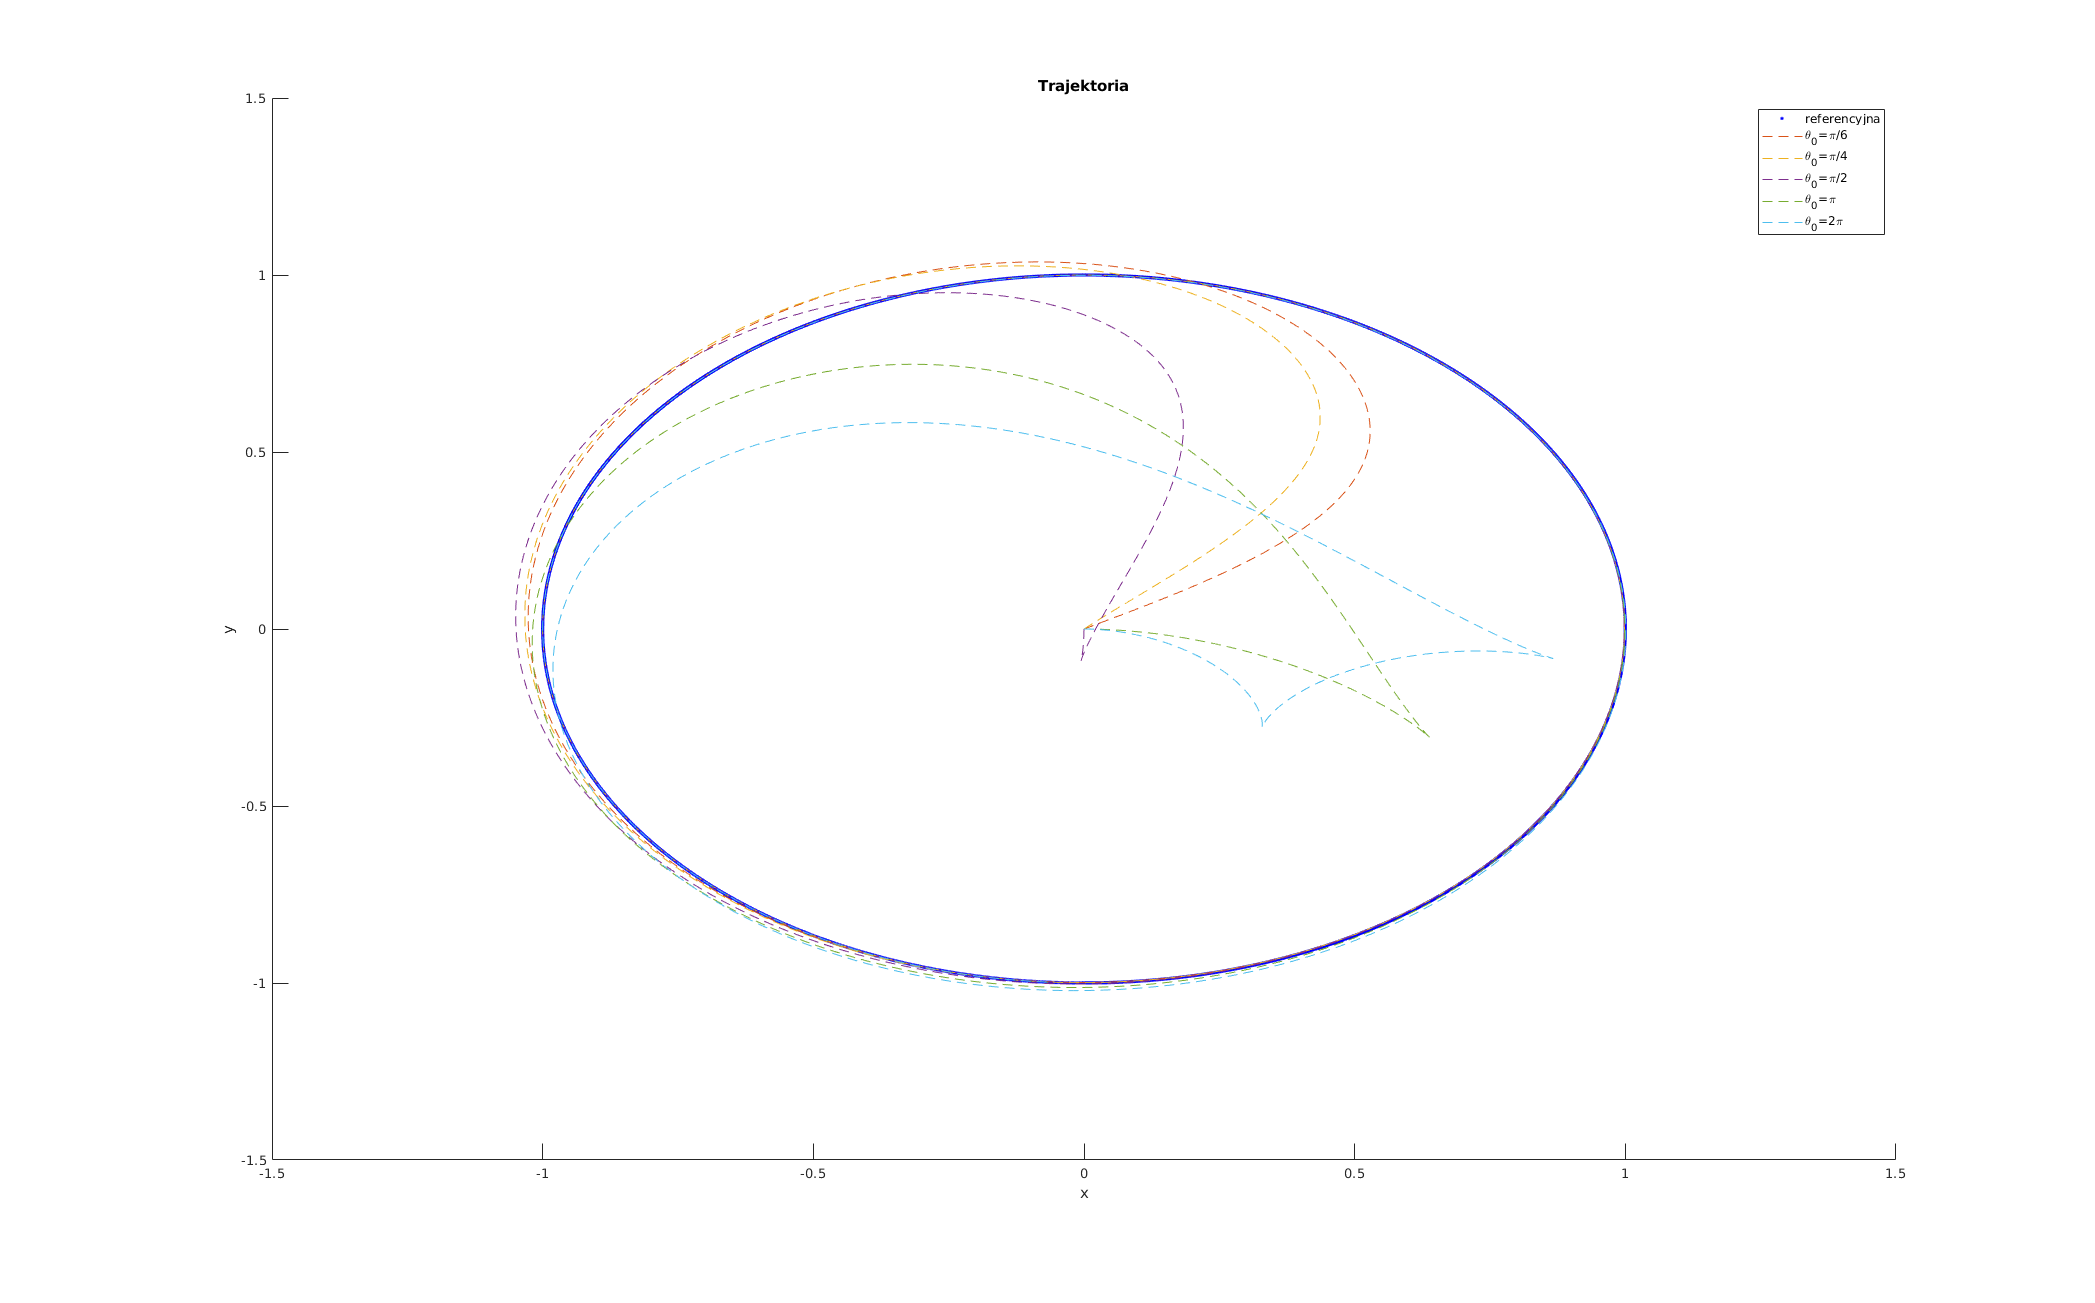
\includegraphics[width=1\textwidth]{figures/wp_o.png}
    \caption{Trajektorie zależne od $\theta_0$}
    \label{fig:13}
  \end{figure}


  \subsection{Wnioski}


  % dlaczego dla platformy musi być kinematyczny i dynamiczny i skąd to się wzięło

  \begin{itemize}
    \item połączenie sterowników powoduje mniejsze opóźnienie i mocniejsze sterowanie,
    \item zmiana współczynnika $K_1$ ma znaczny wpływ na minimalizację błędu $E_x$,
    \item zmiana współczynnika $K_2$ ma znaczny wpływ na minimalizację błędu $E_\theta$,
    \item zmiana współczynnika $K_M$ ma znaczny wpływ na minimalizację błędu $E_x$,
  \end{itemize}
  
\section{Podsumowanie}

  Sterowanie nieholonomicznym obiektem jakim jest platforma mobilna wymaga sterowania przy użyciu sterowanika kinematycznego i dynamicznego. Zadaniem pierwszego algorytmu jest produkcja profilu prędkościowego zależnego od zadania (trajektorii). Następnie informacja ta wykorzystywana jest przez sterownik dynamiczny, który potrafi uwzględnić masę i bezwładność sterowanego obiektu.

\end{document}